\documentclass[12pt,letterpaper]{report}

\usepackage[utf8]{inputenc}
\usepackage[spanish]{babel}
\usepackage{amsmath}
\usepackage{amsfonts}
\usepackage{amssymb}
\usepackage{float}
\usepackage{makeidx} 
\usepackage{graphicx}
\usepackage{color}
%\usepackage{kpfonts} % change font
%\usepackage{mathptmx} % change font
\usepackage{XCharter} % Use the XCharter fonts
\usepackage{multirow}
%\usepackage{natbib}
%\usepackage[numbers]{natbib}
\usepackage[authoryear,comma]{natbib}
%\usepackage{amsmath,amssymb,amsfonts,latexsym,cancel}
\usepackage[left=3cm,right=3cm,top=2cm,bottom=2cm]{geometry}
\usepackage{subcaption}
%\usepackage{url}
\usepackage[breaklinks,colorlinks=true,linkcolor=black,citecolor=black,urlcolor=black]{hyperref}
\usepackage{graphicx}
\usepackage{makecell}
\usepackage{enumitem, hyperref}
\usepackage[table]{xcolor}
\usepackage{longtable}
\usepackage{booktabs}
\usepackage{appendix}
\usepackage{rotating}
\usepackage[spanish,onelanguage,ruled,vlined,lined,resetcount]{algorithm2e}
\SetKw{Break}{finalizar ciclo;}
\usepackage[paper=portrait, pagesize]{typearea}
\usepackage{fancyhdr} % para poner el título en cada capitulo
\usepackage{rotating} % para rotar las paginas
\usepackage{pdflscape}
\usepackage{tablefootnote}
\usepackage{setspace}

\usepackage{vmargin}
\setmargins {2.5cm}       % margen izquierdo
{1.5cm}                        % margen superior
{16.5cm}                      % anchura del texto
{23.42cm}                    % altura del texto
{10pt}                           % altura de los encabezados
{1cm}                           % espacio entre el texto y 			los encabezados
{0pt}                             % altura del pie de página
{2cm} 

% genera el mes de forma automatica
\usepackage{datetime}
\makeatletter
\newdateformat{mifecha}{La Habana, \monthname[\THEMONTH] \THEYEAR}
\renewcommand{\monthnamespanish}[1][\month]{
	\@orgargctr=#1\relax
	\ifcase\@orgargctr
	\PackageError{datetime}{Invalid Month number \the\@orgargctr}{
		Month number should go from 1 to 12
		}
		\or Enero
		\or Febrero
		\or Marzo
		\or Abril
		\or Mayo
		\or Junio
		\or Julio
		\or Agosto
		\or Septiembre
		\or Octubre
		\or Noviembre
		\or Diciembre
		\else \PackageError{datetime}{Invalid Month number \the\@orgargctr}{
			Month number should go from 1 to 12
		}
		\fi
		}


% permite crear listas dentro de lasa tablas
\newcolumntype{e}[1]{%--- Enumerated cells ---
	>{\minipage[t]{\linewidth}%
		\NoHyper%                Hyperref adds a vertical space
		\let\\\tabularnewline
		\enumerate
		\addtolength{\rightskip}{0pt plus 50pt}% for raggedright
		\setlength{\itemsep}{-\parsep}}%
	p{#1}%
	<{\@finalstrut\@arstrutbox\endenumerate
		\endNoHyper
		\endminipage}}

\newcolumntype{i}[1]{%--- Itemized cells ---
	>{\minipage[t]{\linewidth}%
		\let\\\tabularnewline
		\itemize
		\addtolength{\rightskip}{0pt plus 50pt}%
		\setlength{\itemsep}{-\parsep}}%
	p{#1}%
	<{\@finalstrut\@arstrutbox\enditemize\endminipage}}
\makeatother

% esto es para que funcionen los anexos incluyendo la ñ
\makeatletter \renewcommand*{\numberline}[1]{% 
	\hb@xt@\@tempdima{% 
		#1% 
		\protected@edef\@temp@num{#1}% 
		\ifx\@temp@num\@empty\else .\fi \hfil }% 
	} \makeatother


\newenvironment{dedication}
{\clearpage           % we want a new page
	\thispagestyle{empty}% no header and footer
	\vspace*{\stretch{.5}}% some space at the top 
	\itshape             % the text is in italics
	\raggedleft          % flush to the right margin
}
{\par % end the paragraph
	\vspace{\stretch{3}} % space at bottom is three times that at the top
	\clearpage           % finish off the page
}


\title{Nueva versión de componente KNIME para AutoML en tareas de clasificación}

\makeindex 

\renewcommand{\baselinestretch}{1.2}
\begin{document}
	\pagenumbering{roman}	
	\renewcommand{\listtablename}{Índice de tablas}
	\renewcommand{\tablename}{Tabla}
	\renewcommand{\bibname}{Referencias bibliográficas}
	
%	esto es para que las listas anidadas salgan con numeros
	\renewcommand{\labelenumii}{\arabic{enumi}.\arabic{enumii}}
	\renewcommand{\labelenumiii}{\arabic{enumi}.\arabic{enumii}.\arabic{enumiii}}
	\renewcommand{\labelenumiv}{\arabic{enumi}.\arabic{enumii}.\arabic{enumiii}.\arabic{enumiv}}
	
	
	\pagestyle{empty}	
	\markboth{}{} 	
	\thispagestyle{empty} 
	
 	\begin{figure}
	\centering
	
\includegraphics[width=0.5\textwidth]{figuras/membrete-cujae-centrado.png}
\end{figure}
	\begin{center}
	\newcommand{\HRule}{\rule{\linewidth}{0.8mm}}
	
	\vspace*{0.5cm}
	
	\HRule \\[0.4cm]

	\LARGE{\textbf{Nueva versión de componente KNIME para AutoML en tareas de clasificación}}

	\HRule \\[1.5cm]
	
    \textit{\large{Trabajo de diploma para optar por el título de Ingeniería Informática}}

	\vspace{1.5cm}
	
	\large{
	\textbf{Autores:} \\
	Jennifer Yanez Jiménez\\
	Rainer Pellerano Alvarez\\
	\vspace{1.5cm}
	
	\textbf{Tutora:}\\
	Dr. C. Raisa Socorro Llanes\\
	}
	
	\vspace{2cm}
	
	{\mifecha\today}
	
\end{center}	



	\section*{Declaración de autoría}

Declaramos que somos los únicos autores de este trabajo y autorizamos a la Facultad de Ingeniería Informática de la Universidad Tecnológica de la Habana para que haga el uso que estime pertinente de este trabajo. Para que así conste, firmamos la presente a los 3 días del mes de diciembre del año 2023.


\vspace{1cm}

\begingroup	

\setlength{\tabcolsep}{30pt} % Default value: 6pt
\renewcommand{\arraystretch}{0.5} % Default value: 1
\hspace{-1.5cm}
\begin{tabular}{c c}
	
	
\includegraphics[width=0.2\textwidth]{figuras/firmas/firma jenny.png}
	& 
\includegraphics[width=0.3\textwidth]{figuras/firmas/firma ray.png}\\
	Jennifer Yanez Jiménez  & Rainer Pellerano Alvarez \\
	\noindent\rule{6cm}{0.4pt} & \noindent\rule{6cm}{0.4pt} \\ \addlinespace[8pt]
	(Nombre y Apellidos del Diplomante 1) &  		(Nombre y Apellidos del Diplomante 2) 
\end{tabular}
%firma_jpinas
\vspace{5cm}

\hspace{-1.3cm}
\centering
\begin{tabular}{c}
	Dr. C. Raisa Socorro Llanes  \\
	\noindent\rule{6cm}{0.4pt} \\ \addlinespace[8pt]
	(Nombres y apellidos del Tutor) 
\end{tabular}

\endgroup
	\section*{Opinión del tutor}
Lorem ipsum dolor sit amet, consectetur adipiscing elit, sed do eiusmod tempor incididunt ut labore et dolore magna aliqua. Cras tincidunt lobortis feugiat vivamus. Aliquam purus sit amet luctus venenatis lectus magna fringilla. Habitasse platea dictumst quisque sagittis purus sit amet. Vitae et leo duis ut diam quam nulla. Commodo quis imperdiet massa tincidunt. Amet tellus cras adipiscing enim eu turpis egestas. Faucibus ornare suspendisse sed nisi lacus sed. Facilisis leo vel fringilla est ullamcorper eget. Sagittis orci a scelerisque purus semper eget. Netus et malesuada fames ac turpis egestas maecenas pharetra convallis. Quis eleifend quam adipiscing vitae proin sagittis nisl. Enim sit amet venenatis urna cursus eget nunc scelerisque viverra. Ipsum dolor sit amet consectetur adipiscing elit. Ac odio tempor orci dapibus ultrices. Tincidunt vitae semper quis lectus nulla at volutpat diam. Maecenas accumsan lacus vel facilisis volutpat. Tristique sollicitudin nibh sit amet commodo nulla facilisi nullam vehicula. Quis risus sed vulputate odio. Pharetra vel turpis nunc eget lorem dolor sed viverra.

Hac habitasse platea dictumst vestibulum rhoncus est. Suspendisse faucibus interdum posuere lorem. Diam sollicitudin tempor id eu nisl nunc mi. Dignissim diam quis enim lobortis scelerisque. Sed tempus urna et pharetra pharetra massa massa ultricies mi. Urna duis convallis convallis tellus id interdum velit. Viverra ipsum nunc aliquet bibendum enim facilisis. Viverra accumsan in nisl nisi scelerisque eu. Facilisi nullam vehicula ipsum a arcu cursus vitae congue. Aliquet eget sit amet tellus cras adipiscing. Risus ultricies tristique nulla aliquet enim tortor at. Leo urna molestie at elementum eu. Mollis aliquam ut porttitor leo a. Convallis posuere morbi leo urna. Proin fermentum leo vel orci porta non pulvinar. Nulla facilisi morbi tempus iaculis urna id volutpat lacus. Pretium nibh ipsum consequat nisl vel pretium lectus quam id.
	\thispagestyle{empty}
\begin{flushright}
	\begin{minipage}{12.5cm}
		\noindent
		\\[25em]
		%Modificar la cita que se quiere agregar
		%	{\Large Cita 01.}
		%	\\[3em]
		%	Autor
		%	\\ \textit{Fuente}
		%	\\[10em]
		%Para anular la adición de una segunda cita anule las siguientes lineas desde acá mediante comentario (%)
		\begin{flushright}
			\emph{A nuestros familiares y amigos.}
		\end{flushright}		
		%Hasta acá!
	\end{minipage}
\end{flushright} 




	\section*{Agradecimientos de Rainer}
A mi abuela, por ser una madre, muchas gracias, por todo el esfuerzo de criarme, nada fácil de seguro, este trabajo tiene mucho de ti, para no decir casi todo, que no paras de estar orgullosa, aunque no logre nada. Te quiero demasiado mamá. \\
A mi bisabuela, por tanto cariño que me ha dado, por demostrarme que, aunque ya las manos y los pies no den más, hay que seguir obrando, buscar el propósito de vivir. \\
A mi mamá, por el cariño y el amor que me ha dado todos los días, por haberme dado en herencia la parte burlona que me caracteriza, por confiar en mí, gracias. \\
A mi viejo, mi papá, por ser mi ejemplo de esfuerzo, trabajo duro y cuidado de la familia, gracias por apoyarme en todo momento. Dicen que los padres son los más exigentes, pero siempre me dejaste correr por la vida, apoyando mis ideas, mis decisiones, sin ponerme peros, gracias por estar, por guiarme, por quererme. \\
A mi abu, por ser mi referente profesional, por enseñarme que el ser ingeniero, es lo mejor del mundo y que el trabajo para llegar a ello nunca es fácil, por el amor y el cariño, por el tiempo que siempre tienes para cualquier conversación, gracias. \\
A Neni, por ser la que ha pasado todo el proceso a mi lado, en momentos buenos y malos, por darme el amor más grande que he recibido y aguantarme 24 x 24, que eso ya es un mérito, por todos estos años, por alimentarme jaja. Gracias, salchicha Lia. Te amo. \\
A todos los familiares que han formado parte de este proceso, gracias. \\
A Marco, mi hermano, por ser pieza clave en mi vida, que difícil se me hace separarme tanto de alguien que quiero, te extraño demasiado, pero tengo que estar feliz porque tu vida va a mejor, te quiero. La próxima vez que veas al bicho, dile que te firme una camiseta de Messi con las tres estrellas. \\
A Francito y Julito, por ser mi alegría, es verlos y sonrío, gracias por acompañarme todo este tiempo, gracias por los momentazos que siempre pasamos juntos, el cariño que siempre me han dado es impagable, les quiero mucho mis niños. \\
A Miguel, por ser la representación personificada de la fiesta. \\
A mis Guanajos Informáticos: Gordito, por ser lo mejor que he tenido en la carrera, uno aprobado y el otro suspenso no existía, nunca pensé encontrarme familia en la universidad y mira, la próxima carrera que hagamos espero que no esté tan fácil como esta y nos haga estudiar más, gracias por ser mi tándem, gracias por hacerme parte de tu vida (mención especial a la ex casa y a tu hermana que siempre estuvo ahí con nosotros, también te quiero). A Jani por ayudarnos tanto, no hubiese título sin ti, gracias por la paciencia, por la guía, por darnos luz en malos momentos, fuimos a re de numérica por tu culpa, gracias por ser parte fundamental en todo el proceso. A Roi por ser tan s…, tu sabe, siempre fuimos de final de champions. \\
A Jenny, que solo te puedo agradecer y agradecer, no me imaginé que esto fuera tan especial, llenaste algo en mí, que no sé qué es, pero me faltaba, me siento orgulloso de terminar esto a tu lado, me hiciste ser mejor, gracias por haberme acompañado de la mano, te quiero mucho y siempre recuerda \emph{baby, saca esa perra a pasear}. \\
A Raisa, por ser la mejor tutora sacando balones en la línea, gracias por el tiempo que nos dedicas y la sonrisa con la que siempre nos recibe. \\
A mis amigos de aula y a todos los que me ayudaron en algún momento, muchas gracias. \\


	\section*{Resumen}
Vivimos en un mundo en el que se generan grandes cantidades de datos, los cuales se almacenan en diferentes sistemas, y el reto es convertir esos datos en información útil para la toma de decisiones. Una técnica para extraer información valiosa de grandes cantidades de datos es el Aprendizaje Automático, que se enfoca en el desarrollo de modelos y algoritmos que permiten a las computadoras aprender de los datos sin ser programadas explícitamente para hacerlo. Para implementar efectivamente estas técnicas, se requiere de la intervención humana, y la automatización del aprendizaje automático (AutoML) se ha desarrollado como una solución para simplificar y acelerar este proceso. Para ello existen numerosas herramientas, como KNIME, que permite la implementación de AutoML a través de diferentes nodos. En \citep{Carrazana2022} se desarrolla un componente dedicado a esta tarea, específicamente para el pre-procesado en tareas de clasificación. No obstante, quedaron tareas pendientes, como la optimización de hiperparámetros y la automatización de tareas en la fase de transformación de los datos, las cuales son implementadas en la presente investigación. 



\begin{description}
	\item[Palabras clave:]{Aprendizaje Automático, Minería de datos, AutoML, KNIME, optimización de hiperparámetros, preprocesamiento de datos, clasificación.}
\end{description}
%\end{abstract}



	\section*{Abstract}
In a context where the massive generation of data challenges the ability to turn it into valuable information for decision-making, Machine Learning emerges as an essential tool. This approach focuses on developing models and algorithms that enable computers to learn from data without being explicitly programmed to do so. However, the effective implementation of these techniques requires human intervention, and Automated Machine Learning (AutoML) has evolved as a solution to simplify and expedite this process.\\
KNIME, a versatile tool, facilitates the implementation of AutoML through integration with the H2O platform and two AutoML components: the H2O extension, with specific nodes for concrete tasks, and the AutoML Learner component, developed by the KNIME team, which automates the selection of the best algorithm and hyperparameter tuning. Although it offers automation, it lacks the capability for direct control and manual adjustment of processes, thus limiting model customization. On the other hand, there is the AutoML Classification (pre-processing) component, developed at CUJAE by Carrazana (2022), addressing the execution and comparison of AutoML flows in classification tasks with components focused on concise pre-processing tasks. However, the absence of hyperparameter optimization and the lack of automation in essential activities, such as discretization, normalization, handling missing values, and treatment of high cardinality values, pose challenges in data processing and the accuracy of Machine Learning models. \\
This research addresses this gap by proposing a new version of the AutoML Classification (pre-processing) component, where components are created for pre-processing and hyperparameter optimization that, when integrated with the AutoML Classification (pre-processing) component, form the AutoML Classification component. It is demonstrated through its evaluation with five experiments, using five datasets with different characteristics, how with the new implementations an improvement in the performance of the models is achieved, which evidences the system's ability to adapt to different datasets and specific classification needs.

\begin{description}
	\item[Keywords:]{Machine Learning, Data Mining, AutoML, KNIME, HPO, data pre-processing, classification, HPO, hiperparameter optimization}
\end{description}
%\end{abstract}


	

	\markboth{}{}
	\pagestyle{plain}	
	
	\tableofcontents	
	\pagebreak	
	
	\listoftables
	\pagebreak
	
	\listoffigures	
 	\clearpage 
	
	\pagebreak	
	\pagenumbering{arabic}
	
	\phantomsection
	\addcontentsline{toc}{chapter}{Introducción}
	\pagestyle{fancy} 
		
	\fancyhf{}
	\lhead[\thepage]{\textbf{Introducción}}
	\rhead[\textbf{Introducción}]{\thepage}
	
	\chapter*{Introducción}
En la actualidad, en el mundo se generan cada vez mas datos y se almacenan en diversos tipos de sistemas, lo que nos presenta un gran desafío: ¿cómo convertir estos datos en información valiosa que pueda ser utilizada para tomar decisiones informadas? Para resolver este reto, se han desarrollado diversas técnicas y herramientas para extraer información útil de grandes cantidades de datos. \\
El proceso de descubrimiento de conocimiento en bases de datos (\textit{KDD}, por sus siglas en inglés), es un procedimiento que se utiliza para extraer conocimiento útil y relevante, a partir de grandes cantidades de datos almacenados en diversos sistemas \citep{orallo2004}. Este consta de varias fases: integración y recopilación; selección, limpieza y transformación; aplicación de algoritmos de minería de datos; evaluación e interpretación; así como la difusión y uso del conocimiento obtenido \citep{Han2011}. El proceso de descubrimiento de conocimiento en bases de datos ha sentado las bases para una disciplina relacionada, conocida como minería de datos. \\
La minería de datos es el proceso de extraer conocimiento útil y comprensible, previamente desconocido, desde grandes cantidades de datos almacenados en distintos formatos \citep{orallo2004}. Una de las técnicas más comunes de la minería de datos es la clasificación, que consiste en la identificación de un conjunto de categorías o etiquetas para un conjunto de datos no etiquetados \citep{orallo2004}. \\
La clasificación es una técnica muy utilizada en diferentes áreas, como la detección de spam en el correo electrónico \citep{mendez2007sistemas}, la clasificación de imágenes \citep{borras2017clasificacion} y la identificación de transacciones fraudulentas en tarjetas de crédito \citep{dhankhad2018supervised}. Al utilizar algoritmos de clasificación es posible predecir la categoría a la que pertenece un nuevo conjunto de datos, lo que puede ser de gran utilidad en la toma de decisiones y la mejora de los procesos. Esta tarea, a su vez, es uno de los principales enfoques del aprendizaje automático (Machine Learning), una disciplina dentro de la inteligencia artificial, que se basa en la idea de que las computadoras pueden aprender a reconocer patrones y tomar decisiones precisas y acertadas, a través de la experiencia y la retroalimentación continua de los datos. \\
El Aprendizaje Automático se enfoca en el desarrollo de algoritmos y modelos que permiten a las computadoras aprender de los datos sin ser programadas explícitamente para hacerlo. Se define como un conjunto de métodos que puede detectar patrones en los datos automáticamente, y luego usar los patrones descubiertos para predecir datos en el futuro, o para realizar otro tipo de toma de decisiones bajo incertidumbre \citep{murphy2012machine}. Estos patrones interesantes son los que representan el conocimiento. La implementación efectiva de estas técnicas requiere la intervención humana, incluyendo la selección de algoritmos adecuados, el pre-procesamiento de datos y la optimización de hiperparámetros. La Automatización del Aprendizaje Automático (AutoML) se ha desarrollado como una solución para simplificar y acelerar este proceso. \\
 AutoML tiene como objetivo tomar estas decisiones de una manera automatizada, objetiva y basada en datos: el usuario simplemente proporciona datos y el sistema AutoML determina automáticamente el enfoque que funciona mejor para esta aplicación en particular \citep{hutter2019automated}. Para realizar esta tarea de manera efectiva, se requiere de herramientas especializadas que permitan procesar grandes cantidades de información de forma rápida y eficiente. Una de estas herramientas es KNIME.\\
KNIME es una herramienta popular que proporciona un entorno de desarrollo visual para la creación, ejecución y evaluación de flujos de trabajo de análisis de datos. Es una plataforma de software libre y abierto que incluye una amplia variedad de nodos para el pre-procesado de datos, la minería de datos y la modelización de datos \citep{knime2023}. En KNIME, el AutoML se puede implementar a través de una extensión de H2O y dos componentes AutoML; la extensión de H2O, que acoge múltiples nodos para tareas concretas; y el componente \textit{AutoML Learner}, que permite seleccionar automáticamente el mejor algoritmo de aprendizaje automático para un conjunto de datos en particular, así como ajustar los hiperparámetros del modelo. No obstante, una de las principales desventajas que presenta es la falta de control y personalización. Aunque permite a los usuarios seleccionar automáticamente los algoritmos, no tienen control directo sobre estos procesos y no pueden ajustar los parámetros de manera manual. Esto puede limitar la capacidad de los usuarios para personalizar y optimizar los modelos para satisfacer sus necesidades específicas. Mientras, el componente \textit{AutoML (Componente AutoML Clasificación (pre-procesado)} \citep{Carrazana2022}, desarrollado en la CUJAE, ejecuta y compara el desempeño de múltiples flujos de AutoML en tareas de clasificación. En este componente se desarrollaron subcomponentes enfocados en tareas concisas de pre-procesado. Sin embargo, no contempla la optimización de hiperparámetros y la automatización de algunas de las actividades esenciales en el pre-procesado, como discretización y normalización, lo que dificulta el procesamiento de datos y la precisión de los modelos de Aprendizaje Automático. De esta manera se genera un \textbf{problema}: la inexistencia de un nodo en KNIME para AutoML que contenga un pre-procesado completo e incorpore la optimización de hiperparámetros. \\
En aras de resolver la problemática planteada se propone una nueva versión del componente \textit{AutoML (Componente AutoML Clasificación (pre-procesado)} \citep{Carrazana2022}, dado que este permite modificaciones, a diferencia del resto. Por tanto, se determina como \textbf{objetivo general} desarrollar una nueva versión del componente KNIME que permita la selección de manera automatizada de valores e hiperparámetros predefinidos en la implementación anterior. Este objetivo general se desglosa en los siguientes \textbf{objetivos específicos y tareas}:

\begin{enumerate}
	\item Conceptualizar las diferentes categorías que constituyen el centro de la presente investigación.
	\begin{enumerate}
		\item Describir las características del proceso KDD y Minería de Datos. 
		\item Caracterizar las técnicas de Aprendizaje Automático y las principales tareas de Automatización del Aprendizaje Automático.
		\item Asimilar componente AutoML Clasificación (pre-procesado).
	\end{enumerate}
	\item Desarrollar flujos de AutoML en KNIME en tareas de clasificación.
	\begin{enumerate}
		\item Diseñar e implementar subcomponentes en KNIME para la automatización de actividades en el pre-procesado. (En las prácticas profesionales se hará énfasis en la discretización de variables numéricas).
		\item Diseñar e implementar un componente KNIME para la optimización de hiperparámetros.
	\end{enumerate}
	\item Validar subcomponentes de actividades del pre-procesado de datos y componente AutoML Clasificación (Optimización de Hiperparámetros) y su integración al componente AutoML Clasificación (pre-procesado).
	\begin{enumerate}
		\item Diseñar y ejecutar los casos de pruebas que permitan validar los subcomponentes de pre-procesado de datos propuestos. 
		\item Diseñar y ejecutar los casos de pruebas que permitan validar el componente AutoML Clasificación (Optimización de Hiperparámetros).
		\item Diseñar y ejecutar los casos de pruebas que permitan validar la integración del subcomponente de discretización de datos y el componente AutoML Clasificación (Optimización de Hiperparámetros) a el componente AutoML Clasificación (pre-procesado).
		\item Evaluar los resultados arrojados por los casos de prueba.
	\end{enumerate} 
\end{enumerate}

El \textbf{valor práctico} de este proyecto consiste en las modificaciones desarrolladas al componente KNIME de AutoML para el pre-procesado en tareas de clasificación, capaz de automatizar la optimización de hiperparámetros y ejecutar flujos de pre-procesado para diferentes algoritmos en dicha tarea. \\
En cuanto a la estructuración, este trabajo está dividido en tres capítulos:
\begin{itemize}
	\item \textbf{Capítulo 1: Aprendizaje automático y AutoML}, se presenta el estudio realizado sobre las temáticas que aborda el trabajo, se muestran los conceptos fundamentales relacionados con el Aprendizaje automático, la Minería de Datos y AutoML; así como la descripción del componente KNIME de AutoML para pre-procesado.
	\item \textbf{Capítulo 2: Propuesta de modificación al componente KNIME de AutoML para pre-procesado}, se presenta y expone el diseño e implementación de la modificación al componente KNIME para tareas de AutoML en pre-procesado y optimización de hiperparámetros.
		\item \textbf{Capítulo 3: Integración y validación de soluciones propuestas al componente de AutoML}, se muestran, comparan y analizan los resultados obtenidos de los algoritmos para diferentes configuraciones.
\end{itemize}




%Las figuras deben referenciarse en el texto, así como lo muestra este ejemplo, ver Figura \ref{fig:figCUJAE}.

%\begin{figure}[H] %la opción H indica al compilador LaTeX que posicione la figura lo más cerca posible de este lugar.
%\centering
 % 
\includegraphics[width=0.5\linewidth]{figuras/membrete-cujae-centrado.png}
 % \caption{El título de la figura debe estar acorde con su contenido.}
 % \label{fig:figCUJAE} %incluir el label permite referenciarla en cualquier parte del documento.
%\end{figure}

%Se deben utilizar siempre los mismos términos para referirse a los mismos conceptos y no olvidar de definir los términos que son claves en el campo de acción, o sea, la propuesta de la tesis.\\

%Describir la Situación problemática. Problema. Objetivo general. Objetivos específicos. Tareas. Beneficios. Breve resumen del contenido de la tesis.	
	
	\fancyhf{}
	\lhead[\thepage]{\leftmark}
	\rhead[\rightmark]{\thepage}
	\renewcommand{\chaptermark}[1]{\markboth{\chaptername \, \thechapter. #1}{}}
	
	\chapter{Aprendizaje Automático y \textit{AutoML}}\label{chap:1}

En este primer capítulo se aborda el marco teórico de la tesis, el cual se enfoca en diferentes temas clave dentro del campo de la inteligencia artificial y la minería de datos. En particular, se discute el aprendizaje automático, el descubrimiento de conocimiento en bases de datos, la minería de datos y la clasificación. Además, se introduce el concepto de AutoML, como herramienta para automatizar el proceso de preprocesado y optimización de hiperparámetros en la implementación de técnicas de aprendizaje automático. Por último, se destaca la importancia de la plataforma KNIME como una herramienta útil para la implementación de técnicas de AutoML y análisis de datos.

\section{Aprendizaje Automático}
Uno de los campos más destacados dentro de la IA es el Machine Learning (aprendizaje automático), que es un enfoque que utiliza algoritmos y modelos matemáticos para permitir que los sistemas aprendan de los datos y realicen tareas específicas sin ser programados explícitamente.
Se define el Aprendizaje Automático como un conjunto de métodos que pueden detectar automáticamente patrones en los datos y luego usar los patrones descubiertos para predecir datos futuros o para realizar otros tipos de toma de decisiones bajo incertidumbre \citep{murphy2012machine}. Es decir, es el proceso en el que las computadoras descubren cómo hacer cosas sin estar específicamente programadas para hacerlo \citep{Praba2021}.
Por lo tanto, el objetivo principal del aprendizaje automático es estudiar, diseñar y mejorar modelos matemáticos que se pueden entrenar (una vez o continuamente) con datos relacionados con el contexto (proporcionados por un entorno genérico), para inferir el futuro y tomar decisiones sin completo. conocimiento de todos los elementos que influyen (factores externos) \citep{bonaccorso2017machine}. \\
Existen varios tipos de aprendizaje en Machine Learning, cada uno con sus propias técnicas y enfoques. A continuación, se presenta una breve descripción de algunos de los tipos de aprendizaje más comunes:
\begin{itemize}
	\item Aprendizaje supervisado: se refiere a cualquier proceso de aprendizaje automático que aprende una función de un tipo de entrada a un tipo de salida utilizando datos que comprenden ejemplos que tienen valores de entrada y salida. Dos ejemplos típicos de aprendizaje supervisado son el aprendizaje de clasificación y la regresión \citep{sammut2011encyclopedia}. 
	\item Aprendizaje no supervisado: se refiere a cualquier proceso de aprendizaje automático que busca aprender la estructura en ausencia de un resultado identificado o retroalimentación. Tres ejemplos típicos de aprendizaje no supervisado son agrupamiento, reglas de asociación y mapas de autoorganización \citep{sammut2011encyclopedia}. 
	\item Aprendizaje por refuerzo: describe una gran clase de problemas de aprendizaje característicos de los agentes autónomos que interactúan en un entorno: problemas de toma de decisiones secuenciales con recompensa retrasada. Los algoritmos de aprendizaje por refuerzo buscan aprender una política (mapeo de estados a acciones) que maximice la recompensa recibida a lo largo del tiempo \citep{sammut2011encyclopedia}. 
	\item Aprendizaje semisupervisado: es una clase de técnicas de aprendizaje automático que hacen uso de ejemplos etiquetados y no etiquetados al aprender un modelo. En un enfoque, los ejemplos etiquetados se usan para aprender modelos de clase y los ejemplos no etiquetados se usan para refinar los límites entre clases \citep{Han2011}.
\end{itemize}
En resumen, Machine Learning es una técnica que permite a las computadoras aprender patrones a partir de datos, con el objetivo de realizar predicciones o clasificaciones precisas en datos nuevos. Sin embargo, antes de aplicar técnicas de Machine Learning a un conjunto de datos, es necesario realizar una serie de procesos previos, como la selección y preprocesamiento de datos, la selección de técnicas de aprendizaje adecuadas, la evaluación y ajuste de modelos, entre otros. De esta manera, el proceso de  descubrimiento de conocimiento en bases de datos complementa al Machine Learning, permitiendo una exploración más completa de los datos y una selección más adecuada de las técnicas de aprendizaje.

\section{Proceso de descubrimiento de conocimiento en bases de datos}\label{kdd}
La Extracción de Conocimiento en Bases de Datos (\textit{Knwodlege Discovery from Databases}, o \textit{KDD} por sus siglas en inglés) se define como: “el proceso no trivial de identificar patrones válidos, novedosos, potencialmente útiles y, en última instancia, comprensibles a partir de los datos” \citep{orallo2004}. Este proceso está compuesto por una serie de etapas o fases, descritas a continuación:
\begin{itemize}
	\item Integración y recopilación: Se requiere poseer todos los datos que sean de utilidad a partir de las necesidades de la organización. Determina las fuentes de información que pueden ser útiles y dónde conseguirlas. Como parte del desarrollo de esta fase es necesario diseñar o conocer el modo en que se van a organizar e integrar los datos; con el fin de eliminar redundancias e inconsistencias.
	\item Selección, limpieza y transformación: Se seleccionan los datos más relevantes y que aporten mejor información, garantizando que el dato tenga la mejor calidad posible logrando obtener las vistas minables, con los datos listos para la aplicación del algoritmo.
	\item Algoritmos de Minería de datos: A través de la vista minable obtenida en la fase anterior se aplican los algoritmos de extracción del conocimiento.
	\item Evaluación e Interpretación: El objetivo de esta etapa es medir la calidad de los modelos obtenidos utilizando diferentes métricas de calidad. Las cuales dependen de las técnicas de minería de datos que se utilicen. La interpretación de los resultados se apoya en el uso de técnicas de visualización y de representación con el fin de entender mejor el conocimiento aportado. 
	\item Difusión y uso: En esta etapa, se integra el conocimiento obtenido de la comprensión del negocio, con el conocimiento de los modelos de minería de datos usado en la toma de decisiones de los especialistas. La monitorización de los patrones debe realizarse, pues en ocasiones resulta necesaria la reevaluación del modelo, su reentrenamiento o incluso su reconstrucción total.
\end{itemize}
Tras el aumento de  grandes volúmenes de información en toda institución donde se almacenen datos históricos, ahora informatizados en bases de datos digitales, es necesaria la extracción de información valiosa a través de patrones ocultos en estos datos. Sin embargo, esta cantidad de información sobrepasa las capacidades de los analistas de estas instituciones, provocando la necesidad del empleo de técnicas automatizadas. De aquí, surge como una nueva necesidad la minería de datos, siendo parte del proceso KDD.		

\section{Minería de Datos}
Según \citep{orallo2004}, la minería de datos es definida como el proceso de extraer conocimiento útil y comprensible, previamente desconocido, desde grandes cantidades de datos almacenados en distintos formatos. \\
El conocimiento extraído se puede presentar en forma de relaciones, patrones o reglas inferidos de los datos, o en forma de descripción un poco más concisa. Estos constituyen un modelo de datos analizados. Estos modelos, o tareas, se categorizan en predictivas y descriptivas \citep{orallo2004}. \\
En las tareas predictivas, los ejemplos están etiquetados y se emplean para estimar valores futuros o desconocidos de variables de interés. En este entorno se encuentra el aprendizaje supervisado. En cambio, las tareas descriptivas son empleadas en el descubrimiento de propiedades de los datos examinados donde los ejemplos no se encuentran etiquetados. Aquí se pone de manifiesto el aprendizaje no supervisado. En \citep{orallo2004} se describen las tareas de minería de datos como sigue:
\begin{itemize}
	\item Clasificación: La clasificación se encarga de examinar las características de un registro u objeto, y de esta forma asignarle una clase predefinida. Estas clases son valores discretos. Para ello, se tiene que construir un modelo a partir de datos previamente clasificados. Como variantes a la clasificación, existe el aprendizaje de “rankings”, aprendizaje de preferencias y el aprendizaje de probabilidad, entre otros. 
	\item Regresión: A diferencia de la clasificación, el valor a predecir es numérico. Consiste en aprender una función real que calcula un valor para un atributo real. Su objetivo es minimizar el error entre el valor predicho y el valor real.
	\item  Correlaciones: Son empleadas para examinar el grado de similitud de los valores de dos variables numéricas. Se basa en el cálculo de correlación de variables numéricas usando la estadística. Este método trata de determinar si el comportamiento de dos variables numéricas está relacionado.
	\item Reglas de asociación: Las reglas de asociación son situaciones o características que ocurren en un mismo instante de tiempo. Pueden ser relaciones causales o casuales. Representan patrones de comportamiento entre los datos en función de la aparición conjunta de valores de dos o más atributos. Las medidas habituales propuestas en \citep{Agrawal1519}	para establecer la idoneidad y el interés de una regla de asociación son la confianza y el soporte.
	\item	Agrupamiento (Clustering): Para realizar esta tarea se parte de datos sin clasificar, teniendo como objetivo segmentar un grupo de datos diversos en subgrupos. Los miembros de cada grupo (clúster, por su definición en inglés) deben tener mucho en común entre sí y, a su vez, diferenciarse del resto de elementos de otros grupos. Dado que la clasificación de estos grupos no se conoce previamente, es el minero el encargado de darles un significado.
\end{itemize}

\subsection{Clasificación}
En el uso común, la palabra clasificación significa colocar las cosas en categorías, agruparlas de alguna manera útil. Nosotros, como humanos, generalmente hacemos esto porque las cosas en un grupo, llamado \textit{clase} en aprendizaje automático, comparten características comunes \citep{sammut2011encyclopedia}. \\
En aprendizaje automático, la clasificación, se utiliza para identificar a qué clase o categoría pertenece una determinada observación o registro, basándose en un conjunto de características o variables. En esta, se utiliza un algoritmo para construir un modelo predictivo que asigne una etiqueta de clase a cada observación en función de sus características. Este modelo se entrena utilizando un conjunto de datos etiquetados previamente, y luego se aplica a nuevos datos para hacer predicciones \citep{sammut2011encyclopedia}.

\subsubsection{Clasificación con Árboles de Decisión}
La clasificación con árboles de decisión es un método popular en la minería de datos y en el aprendizaje automático supervisado, se utiliza para predecir la clase o categoría de un objeto o registro. Los Árboles de Decisión son unos de los modelos más populares, su representación es de fácil entendimiento, incluso por personas no afines al área, pues su construcción en sencilla: las hojas toman los valores objetivos, mientras los atributos y sus posibles valores conforman los nodos y ramas respectivamente \citep{sammut2011encyclopedia}. \\
Basados en árboles de decisión existen otros algoritmos de clasificación como: ID3, C4.5 y CART. Cada uno de ellos fue desarrollado como una versión mejorada del anterior, pero todos tienen una alta eficiencia y tiempos de ejecución reducidos, lo que los hace igualmente populares en la actualidad \citep{javed2022performance}. Se comparan y analizan en \citep{gupta2017analysis}, donde se arrojan sus principales características:
\begin{itemize}
	\item ID3 (Iterative Dichotomiser 3): Basa su funcionamiento en la entropía y la ganancia de información. El árbol se construye iterativamente de arriba hacia abajo, eligiendo en cada caso el atributo con mayor ganancia de información, hasta que la información ganada sea cero o se haya llegado a todas las hojas \citep{javed2022performance}, \citep{gupta2017analysis}. Maneja datos nominales y no tolera valores faltantes.
	\item C4.5 (Classification 4.5): Desarrollado con el objetivo de mejorar los defectos de ID3. Añade la poda, desestimando las ramas sin aportes, que reduce los errores al clasificar como resultado de un gran número de ramas en el modelo \citep{sammut2011encyclopedia}, \citep{javed2022performance}, \citep{gupta2017analysis}. Adicionalmente maneja valores faltantes y numéricos. 
	\item CART (Classification and Regression Trees): Genera un árbol binario siguiendo el mismo enfoque entrópico que ID3, pero empleando el coeficiente de Gini como criterio de selección \citep{javed2022performance}, \citep{gupta2017analysis}. Es capaz de manejar datos faltantes, al igual que datos numéricos y nominales.
\end{itemize}

\subsubsection{Clasificación con Redes Neuronales}
Las redes neuronales o redes neuronales artificiales, son algoritmos de aprendizaje basados en una vaga analogía de cómo funciona el cerebro humano. El aprendizaje se logra ajustando los pesos en las conexiones entre nodos, que son análogas a las sinapsis y las neuronas \citep{sammut2011encyclopedia}. \\
Las primeras redes neuronales conocidas como pre-alimentadas, como la de la figura \ref{fig:red-neuronal-prealimentada}, se caracterizan por tener una arquitectura en la que cada capa de neuronas está conectada completamente con la capa siguiente, pero no con la capa anterior. Esto significa que la información fluye de forma unidireccional, sin retroalimentación \citep{abiodun2018state}. 
\begin{figure}[H]
	\centering
	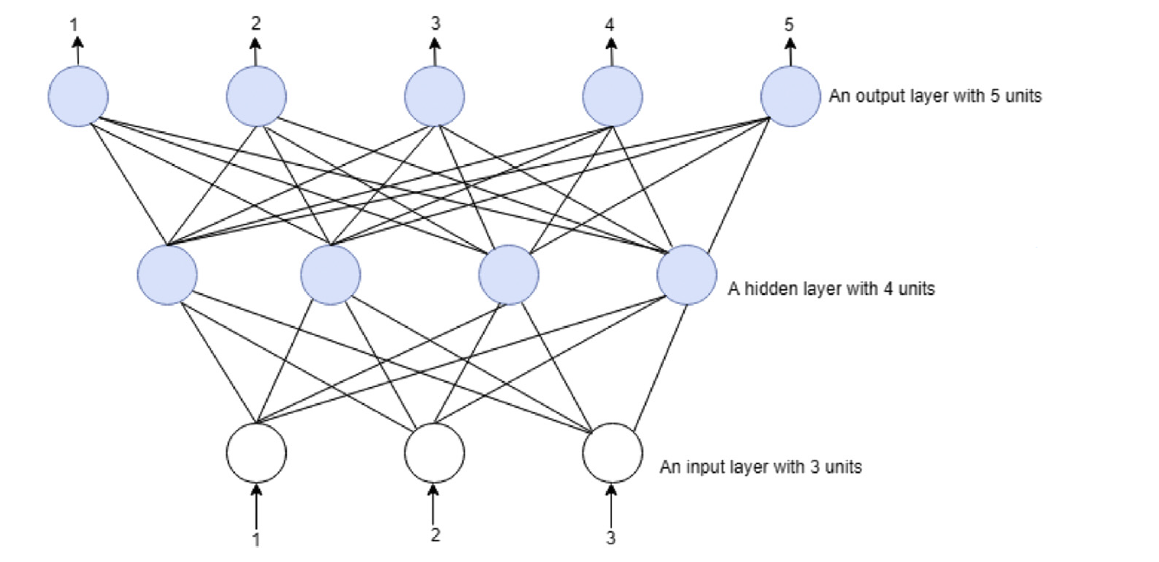
\includegraphics[width=0.7\linewidth]{figuras/capi 1/red-neuronal-prealimentada}
	\caption{Red Neuronal Pre-Alimentada \citep{abiodun2018state}}
	\label{fig:red-neuronal-prealimentada}
\end{figure}
Posteriormente, se desarrollaron las redes neuronales por retro propagación, como la presente en la figura \ref{fig:red-neuronal-retropropagacion}, que comparan la salida obtenida por la red con la salida deseada, y ajustan los pesos de las conexiones entre las neuronas de la red para reducir el error de predicción. La retro propagación se utiliza para calcular la contribución de cada peso en el error de la red, y así ajustarlos de manera adecuada \citep{abiodun2018state}.
\begin{figure}[H]
	\centering
	\includegraphics[width=0.6\linewidth]{figuras/capi 1/red-neuronal-retropropagación}
	\caption{Red neuronal por retro-propagación \citep{abiodun2018state}}
	\label{fig:red-neuronal-retropropagacion}
\end{figure}
Gracias a su gran versatilidad se pueden aplicar en una amplia variedad de campos y disciplinas para resolver problemas complejos de aprendizaje automático, como es el procesamiento del lenguaje natural, reconocimiento de voz e imágenes \citep{abiodun2018state}. Debido a la complejidad de sus modelos puede ser difícil su entendimiento, por lo que preferiblemente se utilizan en el contexto del reconocimiento de patrones, en la figura \ref{fig:red-neuronal-multicapa-compleja} se muestra un ejemplo de Red neuronal multicapa para el reconocimiento facial.
\begin{figure}[H]
	\centering
	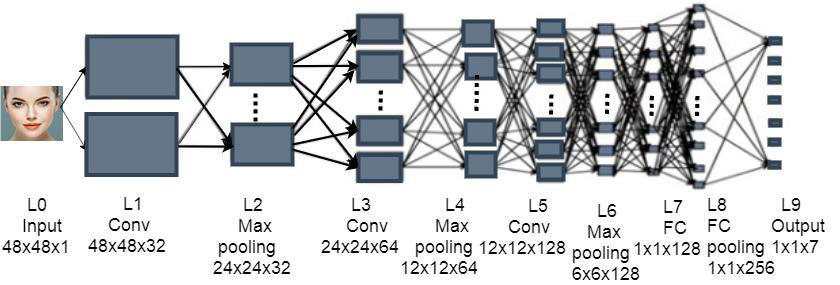
\includegraphics[width=0.7\linewidth]{figuras/capi 1/red-neuronal-multicapa-compleja}
	\caption{Red neuronal multicapa compleja \citep{abiodun2018state}}
	\label{fig:red-neuronal-multicapa-compleja}
\end{figure}

\subsubsection{Clasificación con Support Vector Machine}
Las Máquinas de Soporte Vectorial o Support Vector Machine (SVM) en inglés, son una clase de algoritmos lineales que se pueden usar para clasificación \citep{sammut2011encyclopedia}, cuyo objetivo es encontrar el hiperplano que mejor separa dos clases de datos en un espacio de alta dimensionalidad \citep{guenther2016support}. En la figura \ref{fig:ejemplos-de-posibles-hiperplanos-de-svm} se representa como el hiperplano H2 divide con mayor margen las clases que el hiperplano H1.
\begin{figure}[H]
	\centering
	\includegraphics[width=0.4\linewidth]{"figuras/capi 1/Ejemplos de posibles hiperplanos de SVM"}
	\caption{Ejemplos de posibles hiperplanos de SVM \citep{sammut2011encyclopedia}}
	\label{fig:ejemplos-de-posibles-hiperplanos-de-svm}
\end{figure}
Uno de los desafíos de SVM en problemas de clasificación de múltiples clases es cómo manejar la predicción de estas. En este contexto, existen dos enfoques principales:
\begin{itemize}
	\item Uno contra uno (One-vs-One): Durante la fase de predicción, cada clasificador binario vota por la clase que cree que es correcta y la clase con el mayor número de votos se selecciona como la clase final para el punto de datos dado. Este enfoque presenta la ventaja de que cada clasificador binario solo necesita ser entrenado en un subconjunto de los datos, lo que puede ser útil cuando hay grandes conjuntos de datos. Es más resistente a desequilibrios en la distribución de clases que otros enfoques de SVM \citep{guenther2016support}.
	\item Uno contra todos (One-vs-All): Entrena un clasificador binario para cada clase posible, donde el conjunto de datos de una clase se considera positivo y los datos de las otras clases se consideran negativos. Durante la fase de predicción, cada clasificador binario vota por su clase correspondiente y la clase con la mayor puntuación se selecciona como la clase final para el punto de datos dado. Fácil de implementar y puede funcionar bien en conjuntos de datos pequeños, pero puede ser menos preciso en conjuntos de datos grandes y complejos \citep{guenther2016support}.
\end{itemize}
Agregar que existen otros dos enfoques: Clasificación jerárquica (Hierarchical classification) y Clasificación por parejas (Pairwise classification). Cada uno de estos tiene sus propias ventajas y desventajas, y la elección de uno de ellos dependerá del tipo de datos y del problema que se esté tratando de resolver.

%Texto... Es una buena práctica culminar (o iniciar) cada epígrafe con una referencia al que sigue (o precede) para dar fluidez a su lectura y no se vea como un \emph{copia y pega} sin ninguna relación.
         
\section{\textit{AutoML}}

El campo del aprendizaje automático automatizado (AutoML) tiene como objetivo tomar decisiones de una manera automatizada, objetiva y basada en datos: el usuario simplemente proporciona datos y el sistema AutoML determina automáticamente el enfoque que funciona mejor para esta aplicación en particular \citep{hutter2019automated}. \\
AutoML (Automated Machine Learning) es una técnica que tiene como objetivo automatizar todo o parte del proceso de Machine Learning, incluyendo la selección de algoritmos, la optimización de hiperparámetros, la selección de características y la evaluación del rendimiento del modelo \citep{he2021automl}, \citep{tuggener2019automated}. La relación entre AutoML y Machine Learning es que AutoML es una técnica que se utiliza para automatizar el proceso de Machine Learning, lo que significa que se utiliza para automatizar todo o parte del proceso de selección del mejor modelo de Machine Learning para un conjunto de datos dado. La automatización del proceso de Machine Learning proporciona una solución eficiente y escalable para el análisis de grandes conjuntos de datos, lo que puede resultar en un ahorro significativo de tiempo y recursos para los profesionales de ciencia de datos y los investigadores. \\ 
Tras un análisis del estado del arte acerca del proceso de AutoML \citep{tuggener2019automated}, \citep{waring2020automated}, \citep{hutter2019automated}, \citep{he2021automl}, se pueden presentar las principales tareas como:
\begin{itemize}
	\item Selección de características: Esta tarea consiste en identificar las variables más relevantes para el problema de aprendizaje automático. 
	\item Pre-procesamiento de datos: La calidad de los datos de entrada es un factor crítico en el rendimiento de los modelos de aprendizaje automático. Las técnicas de preprocesamiento de datos se utilizan para limpiar, normalizar y transformar los datos de entrada en un formato que sea adecuado para el modelo. Existen varias técnicas efectivas de preprocesamiento de datos, incluyendo la eliminación de valores atípicos, la imputación de valores faltantes y la normalización y discretización de datos.
	\item Selección de modelo: identificar el modelo de aprendizaje automático que mejor se ajusta al problema dado.
	\item Ajuste de hiperparámetros: Los modelos de aprendizaje automático tienen varios parámetros que afectan su rendimiento, y encontrar los valores óptimos de estos parámetros es una tarea importante para mejorar el rendimiento del modelo. El estado del arte ha demostrado que existen varias técnicas para el ajuste de hiperparámetros, incluyendo la búsqueda aleatoria \citep{zoller2021benchmark} y la optimización bayesiana \citep{he2021automl} \cite{hutter2019automated}.
	\item Evaluación del modelo: La evaluación del modelo es una tarea crítica para medir el rendimiento del modelo en datos de prueba para determinar su capacidad para generalizar. Existen varias técnicas para la evaluación del modelo, incluyendo la validación cruzada y la evaluación de curvas de aprendizaje.
	\item Interpretación del modelo: Analizar el modelo de aprendizaje automático para comprender cómo se toman las decisiones y qué variables son importantes para la predicción.
\end{itemize}

\subsection{Pre-procesado}
Tal como se menciona anteriormente, una tarea importante en el proceso de aprendizaje automático es el pre-procesamiento de datos, que es el conjunto de técnicas utilizadas para preparar los datos de entrada antes de alimentarlos a un modelo de aprendizaje automático. Esta etapa es la equivalente a la fase de selección, limpieza y transformación del proceso de KDD, descrita brevemente en la sección \ref{kdd}. \\
El preprocesamiento de datos ayuda a mejorar la calidad de los datos de entrada y puede mejorar el rendimiento del modelo. La automatización del preprocesamiento de datos a través de herramientas de AutoML puede mejorar la eficiencia del proceso y ayudar al personal especializado, o sin mucha experiencia en el campo, a trabajar de manera más efectiva. Unas de las técnicas de preprocesado de datos son la discretización y la normalización.

\subsubsection*{Discretización}
Este procedimiento transforma datos cuantitativos en datos cualitativos, es decir, atributos numéricos en atributos discretos o nominales con un número finito de intervalos, obteniendo una partición no superpuesta de un dominio continuo. Luego se establece una asociación entre cada intervalo con un valor numérico discreto. Una vez realizada la discretización, los datos pueden ser tratados como datos nominales durante cualquier proceso de minería de datos \citep{garcia2015data}, \citep{garcia2012survey}.

%from you know where%
La discretización se utiliza principalmente para dos propósitos:
\begin{itemize}
	\item Simplificar la información: La discretización reduce la complejidad de los datos continuos, ya que convierte los datos en un número finito de categorías discretas. Esto hace que los datos sean más fáciles de entender e interpretar.
	\item Eliminar la sensibilidad a los valores atípicos: Al discretizar los datos, los valores atípicos se agrupan en una sola categoría discreta, lo que elimina su influencia en el análisis.
\end{itemize}

Existen varias técnicas de discretización, como la discretización por amplitud, la discretización por frecuencia, la discretización por densidad, entre otras. La técnica que se elige depende del tipo de datos y del objetivo del análisis. \\
En la discretización por amplitud, los datos se dividen en un número específico de bins (contenedores) de igual amplitud. En la discretización por frecuencia, los datos se agrupan en bins de forma que cada bin contenga un número aproximadamente igual de observaciones. En la discretización por densidad, los datos se agrupan en bins de forma que cada bin contenga un número aproximadamente igual de densidad de observaciones. \\
La elección de la técnica de discretización y el número de bins a utilizar depende del objetivo del análisis y de la distribución de los datos. Es importante tener en cuenta que la discretización puede introducir cierto grado de pérdida de información, ya que se pierde la precisión de los valores numéricos originales.


\subsubsection*{Normalización}
Este subepígrafe será desarrollado más adelante, durante la redacción de la tesis.

\subsection{Optimización de hiperparámetros}
Cada sistema de aprendizaje automático tiene hiperparámetros, y la tarea básica de AutoML es automatizar el ajuste de estos para maximizar el rendimiento del modelo en un conjunto de datos de prueba o validación \citep{hastie2009elements}. La optimización de hiperparámetros automatizada (HPO) tiene varios casos de uso importantes \citep{hutter2019automated}; puede
\begin{itemize}
	\item reducir el esfuerzo humano necesario para aplicar el aprendizaje automático. Particularmente importante en el contexto de AutoML.
	\item mejorar el rendimiento de los algoritmos de aprendizaje automático (adaptándolos al problema en cuestión).
	\item mejorar la reproducibilidad y equidad de los estudios científicos.
\end{itemize}
Para ahorrar tiempo y mejorar la precisión de los modelos de aprendizaje automático se combina la selección de algoritmos y la optimización de hiperparámetros en un solo proceso, denominado Selección de Algoritmos y Optimización de Hiperparámetros Combinados (CASH por sus siglas en inglés) \citep{tuggener2019automated}. \\
CASH en conjunción con la automatización del pre-procesado de los datos, integran el problema general del AutoML, reflejado en la figura \ref{fig:desglose-de-los-subproblemas-de-automl}. 
\begin{figure}[H]
	\centering
	\includegraphics[width=0.6\linewidth]{"figuras/capi 1/Desglose de los subproblemas de AutoML"}
	\caption{Desglose de los subproblemas de AutoML \citep{zoller2021benchmark}}
	\label{fig:desglose-de-los-subproblemas-de-automl}
\end{figure} 
Existen varias estrategias de HPO, algunas de las cuales son:
\begin{itemize}
	\item Búsqueda aleatoria: Selecciona valores de forma aleatoria dentro de un rango definido. No garantiza encontrar los mejores valores posibles y puede requerir numerosas iteraciones para encontrar un conjunto de hiperparámetros que proporcione un rendimiento óptimo \citep{geron2022hands}, \citep{zoller2021benchmark}.
	\item Búsqueda voraz: Prueba todas las combinaciones posibles de valores de los hiperparámetros dentro de un rango definido. Presenta una alta demanda computacional, imposible de manejar a medida que escalan los sistemas y las bases de datos \citep{zoller2021benchmark}.
	\item Búsqueda en cuadrícula: Prueba cada combinación de valores de hiperparámetros y selecciona la combinación de hiperparámetros que ha dado el mejor rendimiento. Puede ser computacionalmente costoso si el espacio de búsqueda y el número de hiperparámetros es grande \citep{he2021automl}.
	\item Optimización Bayesiana: Construye modelos probabilísticos para representar la función objetivo, que se actualiza después de cada iteración. Maneja espacios de búsqueda de alta dimensionalidad y no requiere tantas iteraciones como la búsqueda en cuadrícula o la búsqueda aleatoria para encontrar combinaciones de hiperparámetros de alto rendimiento \citep{hutter2019automated}, \citep{he2021automl}.
	\item Optimización basada en gradiente: Emplea la información del gradiente para optimizar los hiperparámetros de manera iterativa. Genera una gran carga computacional y presenta la limitación de caer en mínimos locales \citep{zoller2021benchmark}.
\end{itemize} 
A pesar del incesante estudio vinculado al HPO, este sigue presentando en la actualidad diversos desafíos \citep{hutter2019automated}:
\begin{itemize}
	\item Costo computacional: la optimización de hiperparámetros puede ser muy costosa en términos de tiempo de cómputo y recursos de hardware, especialmente cuando se utiliza un espacio de hiperparámetros grande o se ejecutan muchas iteraciones de entrenamiento. Esto puede limitar la escalabilidad y la eficiencia de la HPO.
	\item La generalización del modelo: la optimización de hiperparámetros puede resultar en un modelo altamente ajustado que no generaliza bien a nuevos datos. Se torna complejo cuando las bases de datos poseen múltiples tipos de datos.
	\item Complejidad del espacio de hiperparámetros: el espacio de hiperparámetros puede ser muy complejo y estar altamente interconectado, lo que dificulta la exploración y la selección de los hiperparámetros adecuados.
\end{itemize}
Entre las aplicaciones de HPO se pueden encontrar \citep{hernandeztecnicas}, donde se aplica HPO en SVM y Bosque aleatorio para la Predicción de Enfermedades Cardiovasculares y \citep{waring2020automated}, que manifiesta el desarrollo del problema de HPO en redes Neuronales en un contexto de análisis de salud.
 
\section{Herramienta de minería de datos KNIME}

En la minería de datos se utilizan diferentes herramientas que simplifican el trabajo. KNIME es una de las principales herramientas de minería y análisis de datos, siendo muy completa y ofreciendo muchas funcionalidades \citep{Lisandra2012}. \\
La herramienta de datos KNIME (\textit{Konstanz Information Miner}, por sus siglas en inglés), es una plataforma de minería de datos de código abierto, disponible para varias plataformas y sistemas operativos, que permite el desarrollo de modelos en un entorno visual. Esta herramienta tiene como objetivo desarrollar procesos de KDD a través de un entorno visual. Se le considera una herramienta gráfica, ya que permite construir flujos de trabajo \citep{KNIME2023}. \\
Los flujos se componen de flechas y nodos que se pueden combinar entre sí. Los nodos contienen funcionalidades tales como: algoritmos de minería de datos, formas de conexión a los datos almacenados, preprocesamiento de datos, reportes, entre otros. Las flechas indican el orden de ejecución y el flujo de la información. En la figura \ref{fig:ejemploworkflow} se muestra un ejemplo de un flujo en KNIME para cargar y filtrar datos de una tabla, y posteriormente guardar los resultados en un fichero .csv. 
\begin{figure}[H]
	\centering
	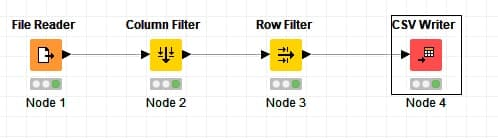
\includegraphics[width=0.9\linewidth]{figuras/capi 1/ejemplo_workflow}
	\caption{Ejemplo de flujo de trabajo en la herramienta KNIME.}
	\label{fig:ejemploworkflow}
\end{figure}

La herramienta KNIME puede ser extendida a través de plugins, la mayoría son nuevos nodos, aunque las extensiones pueden ser a cualquier parte de la arquitectura. La extensibilidad de la herramienta es de forma sencilla, ya que está basada en la Plataforma de Cliente Enriquecido de Eclipse (\textit{Eclipse RCP}, por sus siglas en inglés) \citep{berthold2009knime}. Gracias a esto, la adición de nuevos plugins a KNIME se torna menos compleja para el desarrollador. \\
KNIME se diseñó en base a tres principios: modularidad, extensibilidad y ambiente de trabajo interactivo. A continuación, se describen estos principios \citep{Lisandra2012}:

\begin{itemize}
	\item Modularidad: Plantea que no deben existir dependencias entre las unidades contenedoras de datos o de procesamiento. Además, se pueden implementar algoritmos de manera independiente. De igual forma, al no tener tipos de datos predefinidos, se pueden definir nuevos tipos de datos, con sus características y especificaciones propias. Estos pueden declararse compatibles con otros existentes.
	\item	Extensibilidad de forma sencilla: Permite adicionar nuevas unidades de procesamiento, visualización y tratamiento de datos, teniendo en cuenta que esto debe ser una tarea fácil de realizar.
	\item	Ambiente de trabajo visual e interactivo: Los flujos de trabajo deben ser fáciles e interactivos para el usuario. Por tal motivo, se harán arrastrando los elementos al área de trabajo.
\end{itemize}

Dado que se realiza la modificación de un componente en esta herramienta \citep{Carrazana2022}, se continuará el desarrollo en la misma.

\section{Componente KNIME de AutoML para el pre-procesado en tareas de clasificación}
AutoML en KNIME se refiere a la capacidad de la plataforma para automatizar el proceso de modelado de aprendizaje automático. Esto significa que los usuarios pueden cargar datos y permitir que la plataforma seleccione y optimice automáticamente el modelo que mejor se ajuste a los datos. Con tal objetivo, en \citep{Carrazana2022} se desarrolla un componente Componente KNIME de AutoML para el pre-procesado en tareas de clasificación. Este, a partir de un conjunto de datos y una columna objetivo, ejecuta diferentes flujos de pre-procesado, en aras de cumplir con los requisitos de los diferentes algoritmos de clasificación, siendo capaz de entrenarlos y probarlos, para posteriormente puntuar y graficar los resultados \citep{Carrazana2022}. En la figura \ref{fig:flujo-automl-componente} se muestra el flujo KNIME del componente AutoML Clasificación (pre-procesado).
\begin{figure}
	\centering
	\includegraphics[width=0.8\linewidth]{"figuras/capi 1/flujo-automl-componente"}
	\caption{Flujo KNIME del componente AutoML Clasificación (pre-procesado) \citep{Carrazana2022}}
	\label{fig:flujo-automl-componente}
\end{figure}
Este componente está enfocado en el pre-procesado de datos, donde se desarrollaron subcomponentes enfocados en la realización de las tareas de procesamiento de datos numéricos, string, valores faltantes, y el ajuste de tipos de columna. Como se observa en la figura \ref{fig:flujo-automl-componente}, se aplican los algoritmos de clasificación ID3, C4.5, CART, Redes Neuronales por retro propagación (RProp), Redes Neuronales Probabilísticas (PNN) y Máquina de Soporte Vectorial (SVM). Cada uno de estos requiere un tipo de pre-procesado diferente, acorde a los tipos de datos con los que trabaja. \\
\begin{figure}[H]
	\centering
	\includegraphics[width=0.4\linewidth]{"figuras/capi 1/pre-procesado-id3-ernesto"}
	\caption{Flujo de pre-procesado para el algoritmo ID3 \citep{Carrazana2022}}
	\label{fig:pre-procesado-id3-ernesto}
\end{figure}
No obstante hubo procesos que quedaron pendientes: la optimización de hiperparámetros y la automatización de algunas de las actividades esenciales en el pre-procesado, como la discretización y normalización de variables numéricas. Ambas pueden ser automatizadas acorde a la distribución que sigan los datos, sin embargo están configuradas de forma estática y no toman en cuenta lo anteriormente dicho. Por ejemplo, en la figura \ref{fig:pre-procesado-id3-ernesto} se muestra el nodo AutoBinner, empleado para la discretización, agrupando datos numéricos en intervalos (bins). De igual forma, la optimización de hiperparámetros no fue implementada en esta solución, siendo una de las tareas más importantes en AutoML para mejorar el rendimiento de los algoritmos empleados.

\section{Bases de datos de prueba}
Las bases de datos de prueba son conjuntos de datos creados para ayudar a los desarrolladores a probar y depurar aplicaciones de bases de datos sin tener que utilizar datos reales y confidenciales. Estas bases de datos de prueba contienen datos ficticios, pero siguen la estructura de una base de datos real, lo que permite a los desarrolladores probar la funcionalidad de la aplicación sin preocuparse por dañar datos importantes o comprometer la privacidad de los usuarios. \\
Kaggle Datasets y UCI Machine Learning Repository son dos de los repositorios en línea más populares para conjuntos de datos de prueba y de aprendizaje automático. \\
Kaggle Datasets es un sitio web de aprendizaje automático que ofrece una amplia variedad de conjuntos de datos de muestra, desde datos meteorológicos hasta datos de redes sociales. Los usuarios pueden buscar entre miles de conjuntos de datos y también pueden contribuir con sus propios conjuntos de datos. Kaggle también tiene una comunidad de científicos de datos y aprendizaje automático que pueden proporcionar comentarios y ayudar a los usuarios a mejorar sus modelos de aprendizaje automático. \\
Por otro lado, el UCI Machine Learning Repository es un repositorio de conjuntos de datos de muestra para aprendizaje automático, minería de datos y otras aplicaciones de análisis de datos. El repositorio fue creado por la Universidad de California, Irvine y contiene una amplia gama de conjuntos de datos, desde reconocimiento de voz hasta predicción de precios de viviendas. Los usuarios pueden descargar los conjuntos de datos de forma gratuita y utilizarlos para probar y desarrollar sus modelos de aprendizaje automático. \\
Ambos repositorios ofrecen una amplia variedad de conjuntos de datos, lo que los hace ideales para desarrolladores, estudiantes y profesionales de la ciencia de datos que buscan mejorar sus habilidades en el modelado de bases de datos y en la creación de modelos de aprendizaje automático precisos y efectivos. Por tal motivo, se emplearán ambos repositorios para la obtención de bases de datos para las pruebas que se realizarán más adelante.


\section{Conclusiones parciales}

% Cada conclusión tiene que estar sustentada en el cuerpo del capítulo.

A partir de lo estudiado en este capítulo, se llega a las siguientes conclusiones:

\begin{itemize}
	\item El Aprendizaje Automático es una técnica que permite a las computadoras aprender a partir de datos, sin necesidad de ser programadas explícitamente.
	\item El proceso de descubrimiento de conocimiento en bases de datos (KDD) es un proceso iterativo que consiste en varias etapas, incluyendo la selección de datos, la limpieza de datos, la transformación de datos y la minería de datos.
	\item La Minería de Datos es el proceso de descubrir patrones y relaciones interesantes en grandes conjuntos de datos, utilizando técnicas de aprendizaje automático, estadísticas y visualización de datos. Algunas de las técnicas utilizadas en la Minería de Datos incluyen la clasificación, la agrupación, la regresión y la asociación.
	\item La Clasificación es una técnica de aprendizaje automático que se utiliza para predecir la etiqueta o clase de un objeto a partir de un conjunto de características.
	\item El AutoML se puede utilizar para mejorar la eficiencia y la precisión del proceso de modelado, reducir la necesidad de conocimientos especializados y permitir a los usuarios enfocarse en la interpretación de los resultados. Las etapas del AutoML incluyen la selección automática de algoritmos, el preprocesamiento de datos, la optimización de hiperparámetros y la evaluación automática del modelo.
	\item El preprocesamiento de datos es una etapa crítica en el proceso de modelado, ya que los datos deben limpiarse, integrarse y transformarse antes de ser utilizados por los algoritmos de aprendizaje automático.
	\item Algunas de las tareas comunes del preprocesado de datos incluyen la eliminación de valores atípicos, el manejo de datos faltantes, la discretización y la normalización de datos numéricos.
	\item La discretización es una técnica utilizada para transformar datos numéricos en datos categóricos.
	\item Los hiperparámetros son ajustes que se realizan en los algoritmos de aprendizaje automático para mejorar su rendimiento. La optimización de hiperparámetros implica encontrar la combinación óptima de valores para los hiperparámetros.
	\item KNIME es una herramienta de minería de datos de código abierto que permite a los usuarios crear y ejecutar flujos de trabajo de análisis de datos.
\end{itemize}


%Una vez terminado el capítulo se arriban a las siguientes conclusiones:

%\begin{enumerate}
%	\setlength\itemsep{0em}
%	\item Una conclusión necesaria aquí son los requisitos principales que debe cumplir la solución propuesta.
%	\item Otra conclusión es la inexistencia de una solución que brinde cumplimiento a los requisitos planteados.
%	\item Finalmente, cuáles son las tecnologías seleccionadas y su justificación
%\end{enumerate}

\pagebreak

	\chapter{Propuesta de modificaciones al componente AutoML para pre-procesado}\label{chap:2}
En el presente capítulo, se propone una serie de modificaciones destinadas a mejorar el componente \emph{AutoML Clasificación (pre-procesado)}. Estas modificaciones se centran en el pre-procesamiento de datos, incluyendo la automatización de tareas como la discretización, normalización y el tratamiento de valores únicos, valores de alta cardinalidad y valores faltantes. Además, se explorará la inclusión de técnicas de Optimización de Hiperparámetros (HPO) para encontrar configuraciones óptimas para los modelos. El enfoque principal de esta propuesta es la integración de estas dos facetas con el componente AutoML existente para clasificación. A lo largo de este capítulo, se describirá cómo estas modificaciones buscan mejorar la eficiencia y precisión del proceso de AutoML, creando modelos de clasificación más sólidos y adaptados a las necesidades específicas de los datos.

\section{Modificaciones en el pre-procesado}
Con el fin de abordar las problemáticas presentadas en el subepígrafe \ref{sec:componente-knime-de-automl-clasificacion-pre-procesado}, es decir, la falta de automatización de la discretización y normalización, el tratamiento de valores únicos, valores de alta cardinalidad y valores faltantes, se llevaron a cabo una serie de modificaciones sustanciales en el proceso de pre-procesamiento de datos. \\
 En lo que respecta a la discretización y normalización, se implementaron técnicas automatizadas para garantizar una uniformidad en la escala y distribución de los datos, lo que contribuye a mejorar la precisión del modelado. Para abordar los valores únicos y de alta cardinalidad, se desarrollaron estrategias específicas que permitieron una gestión más efectiva de estas categorías, evitando la pérdida de información esencial y reduciendo el riesgo de sobreajuste. Por último, se implementaron métodos especializados para tratar los valores faltantes, asegurando que los datos incompletos no comprometieran la calidad del análisis. En los epígrafes siguientes, se detalla el funcionamiento y modelado de estas modificaciones con mayor profundidad. Para ello, se crean componentes con el objetivo de integrarse al componente\textit{ AutoML Clasificación (pre-procesado)}.

\subsection{Discretización de variables numéricas} 
La discretización de variables numéricas se utiliza para convertir datos continuos en datos discretos, lo que permite que los algoritmos de aprendizaje automático puedan procesarlos y analizarlos adecuadamente. La discretización también puede mejorar la precisión de los modelos de aprendizaje automático al reducir el ruido en los datos y hacer que los patrones sean más fáciles de detectar. En aras de automatizar este proceso, se propone el componente \textit{Discretizer}. \\
El componente \textit{Discretizer} toma en su puerto de entrada los datos en formato tabular. Dichos datos, de tipo numéricos, son procesados por varios algoritmos de discretización y, como puerto de salida, se obtienen discretizados acorde al método de discretización con mejor precisión. Tiene una única restricción: no pueden tener valores perdidos como entrada. El diagrama de flujo de la Figura \ref{fig:discretizacion} expone el flujo general del componente \textit{Discretizer}. El flujo KNIME correspondiente está presente en el Anexo \ref{aped:8}. 

\begin{figure}[H]
	\centering
	\includegraphics[width=1\linewidth]{"figuras/capi 2/preprocesado/discretizacion.drawio"}
	\caption{Diagrama de flujo general de \textit{Discretizer}}
	\label{fig:discretizacion}
\end{figure}

Para la discretización se emplean los nodos presentes en la Figura \ref{fig:discretizacion-nodos}. El nodo \textit{Auto-Binner} contiene tres métodos de discretización: \textit{Equal-Width, Equal-Frequency} (Anexo \ref{aped:9}) y \textit{Quantile-Based}; mientras el nodo \textit{CAIM Binner} contiene el método \textit{CAIM}. Para la elección de los \textit{k} intervalos se emplea la Regla de Sturges, descrita en el epígrafe \ref{sub-epigrafe-disc}, debido a su sencilla implementación en la herramienta. El nodo \textit{CAIM Binner} no requiere una configuración en específico, y para el método \textit{Quantile-Based} se escogieron los cuantiles 0.0, 0.25, 0.5, 0.75 y 1.0. Esta decisión se basa en varios aspectos como:
\begin{enumerate}
	\item Distribución de los datos: para capturar diversos puntos en la distribución de los datos. Estos cuantiles proporcionan una representación equitativa de la variabilidad de los valores en el conjunto de datos. El cuantil 0.0 representa el valor mínimo, el cuantil 1.0 representa el valor máximo y los cuantiles 0.25, 0.5 y 0.75 dividen los datos en cuartiles. Esta selección asegura que se están considerando tanto los extremos como los valores centrales de la distribución.
	\item Robustez ante valores atípicos: la elección de estos cuantiles también está respaldada por la necesidad de que los modelos sean robustos ante valores atípicos. Los cuantiles 0.0 y 1.0 permiten considerar directamente los valores mínimos y máximos, lo que puede ser crítico para lidiar con datos extremos que pueden afectar significativamente el rendimiento de nuestros modelos.
	\item Interpretabilidad: para mejorar la interpretabilidad de los resultados, se opta por seleccionar los cuantiles 0.25, 0.5 y 0.75, que representan los cuartiles. Los cuartiles son puntos de referencia bien conocidos en estadísticas y facilitan la comunicación de resultados a personas no técnicas. 
	\item Consistencia y comparabilidad: utilizar cuantiles específicos como 0.0, 0.25, 0.5, 0.75 y 1.0 puede hacer que los resultados sean más consistentes y comparables entre diferentes análisis o modelos, ya que se utilizan puntos de corte estándar en la distribución de los datos.
\end{enumerate}

\begin{figure}[H]
	\centering
	\begin{subfigure}[b]{0.25\linewidth}
		\centering
		\includegraphics[width=0.5\linewidth]{"figuras/capi 2/auto-binner-nodo"}
		\caption{Nodo \textit{Auto-Binner}}
		\label{fig:auto-binner-nodo}
	\end{subfigure}
	\hspace{1.5cm}
	\begin{subfigure}[b]{0.25\linewidth}
		\centering
		\includegraphics[width=0.5\linewidth]{"figuras/capi 2/caim-binner-nodo"}
		\caption{Nodo \textit{CAIM Binner}}
		\label{fig:caim-binner-nodo}
	\end{subfigure}
	\caption{Nodos empleados para la discretización}
	\label{fig:discretizacion-nodos}
\end{figure}

Tras discretizar el conjunto de datos con cada método correspondiente, se aplica el modelo en cuestión a cada uno de los datos resultantes, con el objetivo de compararlos en cuanto a las métricas Exactitud y Cohen's Kappa, y escoger el algoritmo con mejor desempeño. Estas métricas se emplean debido que son brindadas por el nodo \textit{Scorer} de KNIME, que tiene como objetivo la evaluación de modelos de clasificación; además proporcionan una visión general del rendimiento del modelo sin importar si se trata de un problema de naturaleza binaria o multiclase. Se toma en cuenta la exactitud y, en caso de empate, el Cohen's Kappa. Este esquema de comparación se continúa empleando a lo largo de este estudio.

\subsection{Pre-procesado de variables de tipo \textit{string}}
Los valores nominales únicos, o categorías con un solo ejemplo en una columna, pueden parecer insignificantes a primera vista, pero su correcto manejo es esencial para evitar posibles problemas de calidad de datos y garantizar la integridad de los análisis. El componente \textit{AutoML Clasificación (pre-procesado)} poseía un tratamiento erróneo de estos valores al eliminar las columnas nominales que contenían un número de categorías diferentes que superaban un umbral. Este umbral era determinado por el usuario en la configuración del componente. \\ 
En aras de depurar estas inconsistencias, el diagrama de la Figura \ref{fig:string-preprocs} muestra un nuevo flujo para el pre-procesado de \textit{string}, donde la actividad de color amarillo expresa que se modificó la que anteriormente se encontraba en el componente; mientras que la actividad en verde refleja una nueva implementación.

\begin{figure}[H]
	\centering
	\includegraphics[width=0.95\linewidth]{"figuras/capi 2/preprocesado/string preprocs.drawio"}
	\caption{Diagrama de flujo para el pre-procesado de \textit{string}}
	\label{fig:string-preprocs}
\end{figure}

A continuación se exponen los cambios realizados al componente \textit{String preprocs}:
\begin{itemize}

	\item Eliminar valores únicos por columna: se enmienda el error antes expuesto, al modificar el componente \textit{Filtrar valores únicos}, implementando la eliminación de las columnas donde más del 80\% de los valores son únicos. En la Figura \ref{fig:filtrar-valores-unicos-flujo} se muestra una parte del flujo KNIME donde se implementa esta tarea. 

	\begin{figure}[H]
		\centering
		\includegraphics[width=0.9\linewidth]{"figuras/capi 2/preprocesado/filtrar-valores-unicos-flujo"}
		\caption{Vista previa de flujo KNIME para el filtrado de valores únicos}
		\label{fig:filtrar-valores-unicos-flujo}
	\end{figure}

	\item Reemplazar con otros: en este nuevo componente, los valores únicos en una columna que representan una minoría, son reemplazados por la categoría '\textit{other}'.  Para ello, iterando por cada columna dentro de un ciclo, se calculan la frecuencia absoluta y relativa de cada atributo (nodo \textit{Math Formula}), y aquellos que representen menos del 1\% son los elegidos para la sustitución por la nueva categoría (nodo \textit{Java Snippet}). En la Figura \ref{fig:flujo-reemplazar-others} se muestra una parte del flujo KNIME donde se implementa esta tarea. 

	\begin{figure}[H]
		\centering
		\includegraphics[width=1\linewidth]{"figuras/capi 2/preprocesado/flujo-reemplazar-others"}
		\caption{Vista previa de flujo KNIME para el reemplazo por '\textit{other}'}
		\label{fig:flujo-reemplazar-others}
	\end{figure}

	
\end{itemize}


\subsection{Manejo de valores faltantes}
El tratamiento de valores faltantes en conjuntos de datos es un paso crítico en la preparación y análisis de datos. La presencia de datos faltantes puede afectar significativamente la calidad y la fiabilidad de cualquier análisis o modelo que se derive de ellos. Adicionalmente, algunos algoritmos requieren que no existan valores faltantes para su funcionamiento. En aras de mejorar la imputación de estos valores, se propone modificar el componente \textit{Valores faltantes}, cuyo diagrama de flujo se presenta en la Figura \ref{fig:valores-faltantes}.

\begin{figure}[H]
	\centering
	\includegraphics[width=1\linewidth]{"figuras/capi 2/preprocesado/valores faltantes.drawio"}
	\caption{Diagrama de flujo para el manejo de valores faltantes}
	\label{fig:valores-faltantes}
\end{figure}

La imputación de valores faltantes ha sido modificada, dado que anteriormente se sustituían por la media los valores faltantes numéricos, y por la moda los atributos categóricos. En la Figura \ref{fig:mv-imputation} se presenta el diagrama de flujo de la nueva implementación para la sustitución de estos valores. El flujo KNIME correspondiente está presente en el Anexo \ref{aped:10}. 

\begin{figure}[H]
	\centering
	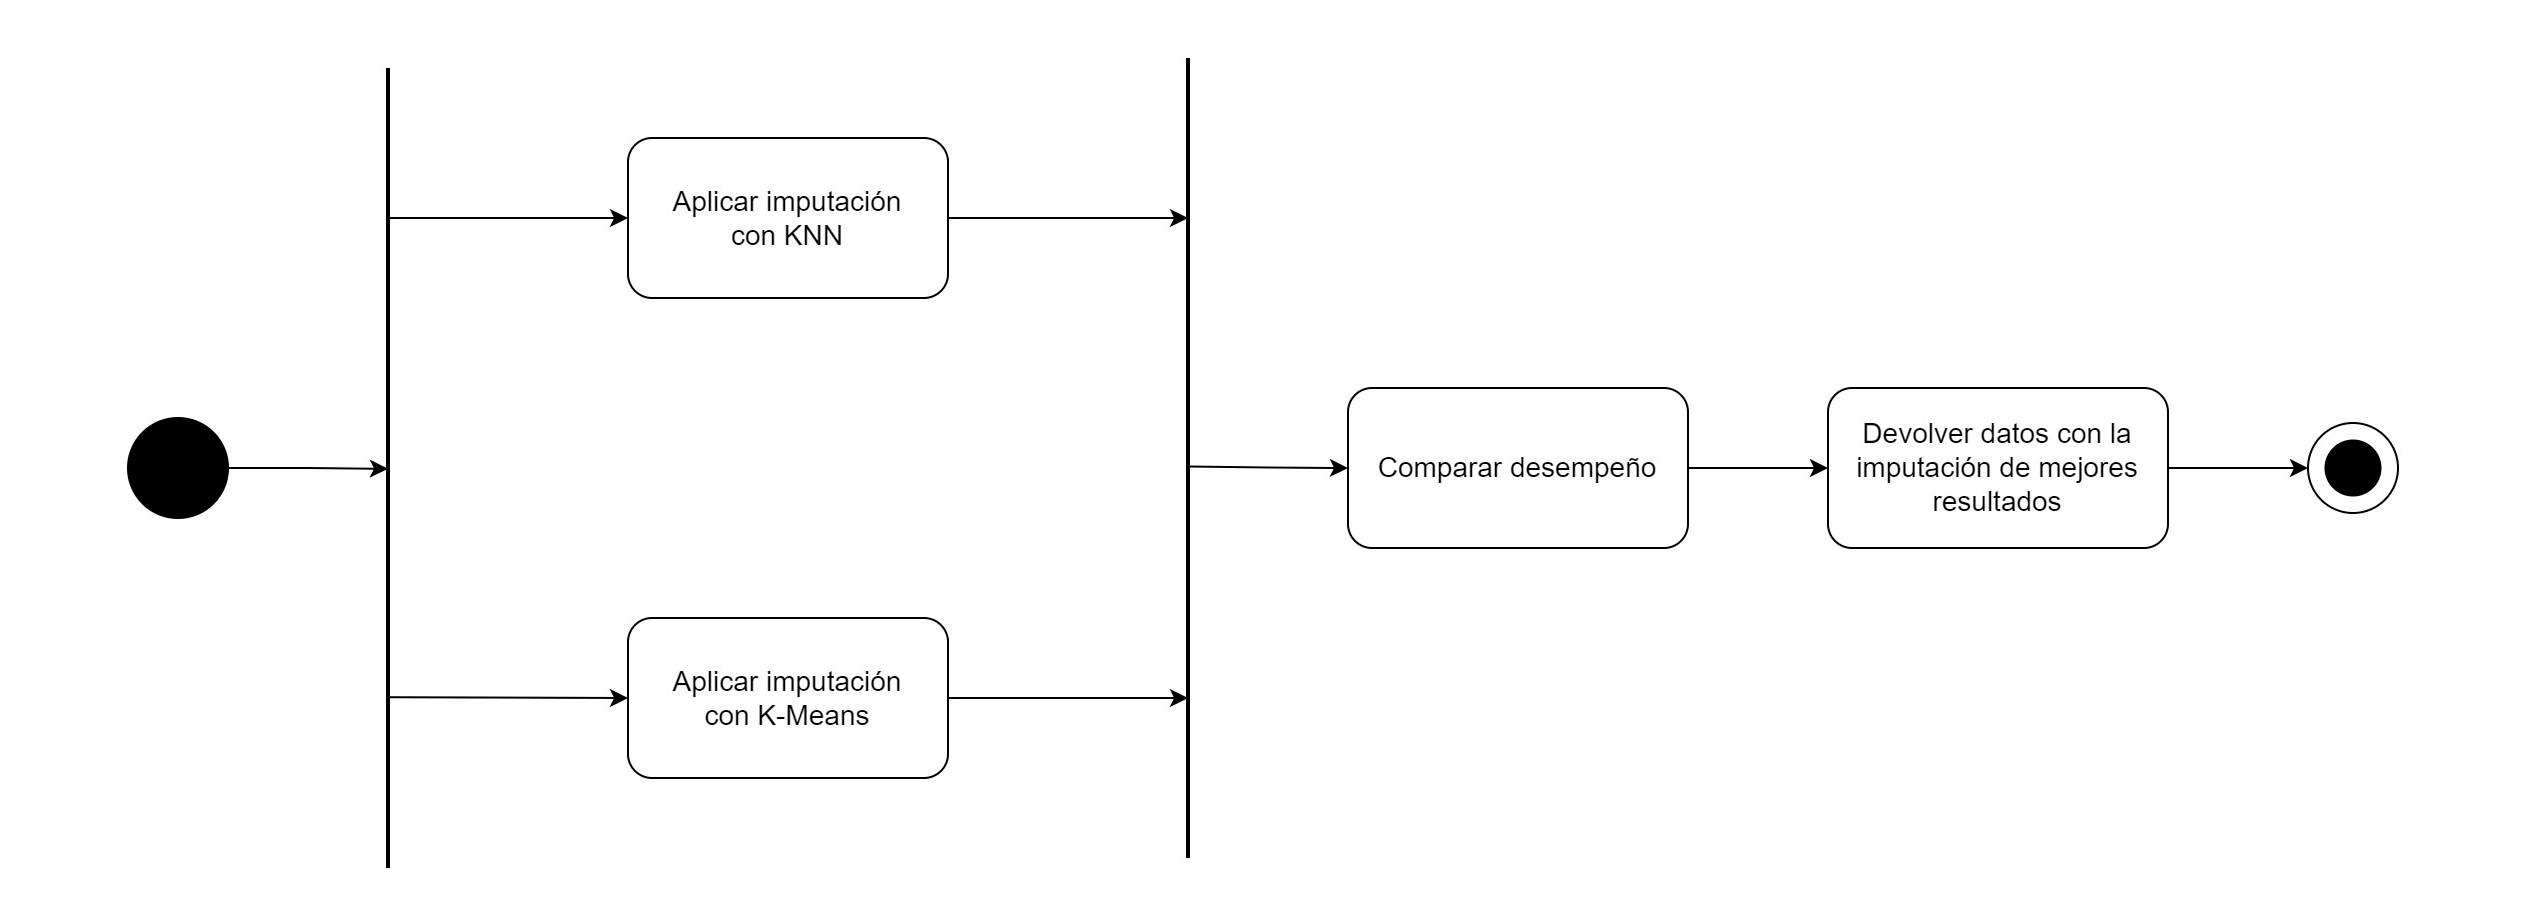
\includegraphics[width=1\linewidth]{"figuras/capi 2/preprocesado/mv imputation.drawio"}
	\caption{Diagrama de flujo para la imputación de valores faltantes}
	\label{fig:mv-imputation}
\end{figure}

Primeramente se aplican en paralelo las técnicas de imputación kNN y k-Means, al terminar se aplica el algoritmo de aprendizaje automático en cuestión con los datos imputados por cada método y, finalmente, se comparan los resultados acorde al esquema descrito en el componente \textit{Discretizer} para devolver los datos con la mejor sustitución. \\
Para la implementación de kNN y k-Means, se crearon dos subcomponentes: kNNI (\textit{k-Nearest Neighbors Imputation}) y kMI (\textit{k-Means Imputation}). Se emplean los nodos \textit{kNN} y \textit{k-Means}, ambos nativos de KNIME. Para escoger \textit{k}, en k-Means se utiliza el Método de la Silueta, ya que KNIME contiene el nodo \textit{Silhouette Coefficient}; mientras que para kNN se decide emplear la raíz cuadrada de la muestra, debido a su simpleza en la implementación y que este método podría ofrecer cierta estabilidad en la elección del número de vecinos, independientemente del tamaño específico del conjunto de datos. Esto podría hacer que el modelo sea menos sensible a variaciones en el tamaño de la muestra. A continuación se describe el funcionamiento de k-NNI y kMI:

\begin{itemize}
	\item kMI:
	\begin{enumerate}
		\item Convertir los valores nominales en numéricos para que el nodo trabaje con ellos, ya que este algoritmo solamente trata este tipo de valores.
		\item Separar las columnas con valores perdidos para que el algoritmo pueda realizar el proceso de \textit{clustering} con los datos sin estos valores, ya que no los tolera el nodo.
		\item Calcular valor óptimo de \textit{k} con el Método de la Silueta.
		\item Aplicar k-Means a estos datos.
		\item Unir las columnas que contienen valores perdidos con los datos etiquetados con su respectivo clúster.
		\item Aplicar el nodo \textit{Missing Value}, nativo de KNIME, tras filtrar por clúster, sustituyendo los valores perdidos por la media de esa columna, es decir el valor del centroide de ese clúster.
		\item Retornar las variables numéricas a categóricas (las que se transformaron inicialmente) para recuperar su valor original.
	\end{enumerate}
	\item kNNI:
	\begin{enumerate}
		\item Convertir los valores nominales en numéricos para que el nodo trabaje con ellos, ya que este algoritmo solamente trata este tipo de valores.
		\item Extraer los nombres de las columnas que contienen valores perdidas.
		\item Por cada columna, se separan los valores perdidos del resto de los datos, éstos se reemplazan por 0 si son numéricos, si son de tipo \textit{string} se ignoran.
		\item Calcular el valor de \textit{k} mediante la raíz cuadrada de la muestra. 
		\item Los datos sin valores perdidos se emplean para el entrenamiento de kNN, mientras los datos con estos se emplean para la predicción.
		\item Retornar las variables numéricas a categóricas (las que se transformaron inicialmente) para recuperar su valor original.
	\end{enumerate}
\end{itemize}

 En las Figuras \ref{fig:flujo-knni} y \ref{fig:flujo-kmi} se muestran los flujos de trabajo que se implementan para la imputación con los algoritmos kNNI y kMI, respectivamente.
 
 \begin{figure}[H]
 	\centering
 	\includegraphics[width=0.9\linewidth]{"figuras/capi 2/preprocesado/flujo-knni"}
 	\caption{Vista previa de flujo KNIME para kNNI}
 	\label{fig:flujo-knni}
 \end{figure}
 
  \begin{figure}[H]
 	\centering
 	\includegraphics[width=0.9\linewidth]{"figuras/capi 2/preprocesado/flujo-kmi"}
 	\caption{Vista previa de flujo KNIME para kMI}
 	\label{fig:flujo-kmi}
 \end{figure}
 
 

\subsection{Codificación y normalización}
La codificación de variables categóricas implica asignar valores numéricos a estas categorías para que los algoritmos de aprendizaje automático puedan trabajar con ellas. Este es el propósito del componente \textit{Pre-procesar números}, además de la normalización de variables numéricas. En aras de clarificar el funcionamiento de este proceso, se decide renombrarlo a \textit{Codificar y normalizar}.\\
La normalización son proporciones sin unidades de medida (adimensionales o invariantes de escala) que nos permiten poder comparar elementos de distintas variables y unidades de medida. Esta es necesaria para cambiar los valores de las columnas numéricas del conjunto de datos para usar una escala común, sin distorsionar las diferencias en los intervalos de valores ni perder información. La normalización es fundamental para que algunos algoritmos modelen los datos correctamente. \\
En KNIME es posible implementar la normalización a partir del nodo \textit{Normalizer}. En este nodo se encuentran tres métodos para normalizar, a elección del usuario: \textit{Decimal Scaling, Z-Score y Min-Max}. Este proceso se encuentra en el componente para el pre-procesado de números, cuyo diagrama de flujo se presenta en la Figura \ref{fig:number-preprocs}. El flujo KNIME correspondiente está presente en el Anexo \ref{aped:11}. 

\begin{figure}[H]
	\centering
	\includegraphics[width=1\linewidth]{"figuras/capi 2/preprocesado/number preprocs.drawio"}
	\caption{Diagrama de flujo del pre-procesado para la codificación y normalización}
	\label{fig:number-preprocs}
\end{figure}
Por otro lado, los valores de alta cardinalidad, aquellos que se repiten con frecuencia y pueden ser numerosos, son cruciales para comprender tendencias y patrones en los datos. La codificación de estas variables se refiere a técnicas especiales de codificación que se utilizan cuando se tienen variables categóricas con un gran número de categorías o niveles distintos. La alta cardinalidad puede dificultar la gestión de estas variables en modelos de aprendizaje automático, y es importante abordarlas de manera eficiente. \\ 
A continuación se exponen los cambios realizados al pre-procesado para la codificación y normalización:

\begin{itemize}

	\item Codificar con \textit{One-Hot Encoding}: para el tratamiento de valores con alta cardinalidad, se emplea la codificación One-Hot (ver subepígrafe \ref{alta-cardinalidad}), ya que KNIME brinda el nodo \textit{One To Many} para esta tarea. Para esto se escogen los atributos que tienen como mínimo 15 categorías distintas. \textit{One-Hot Encoding} se utiliza para codificar variables categóricas en una forma que no impone un orden implícito en las categorías. Cuando se tienen más de 15 categorías, es poco probable que haya un orden natural o jerarquía en esas categorías, por lo que codificarlas como variables binarias evita interpretaciones erróneas de orden o importancia. Dado que esta técnica produce gran dimensionalidad, se utiliza para su reducción el método PCA, con un límite de conservación de la información del 90\%. Este proceso se encuentra implementado en la Figura \ref{fig:one-hot-flujo}.
	
	\begin{figure}[H]
		\centering
		\includegraphics[width=1\linewidth]{"figuras/capi 2/preprocesado/one-hot-flujo"}
		\caption{Vista previa de flujo KNIME para la codificación One-Hot}
		\label{fig:one-hot-flujo}
	\end{figure}
	
	\item Normalizar: con el propósito de automatizar este proceso, se propone el componente \textit{Normalizer}, de igual nombre al nodo nativo de KNIME, en donde se encuentra el mismo para la ejecución de los métodos que contiene, en función de un modelo predeterminado. En la Figura \ref{fig:normalizacion} se presenta el diagrama de flujo de este componente. En el Anexo \ref{aped:12} se muestra un ejemplo de implementación de un flujo KNIME para la normalización, en este caso, empleando el método \textit{Decimal Scaling}, para el modelo PNN.

\end{itemize}

\begin{figure}[H]
	\centering
	\includegraphics[width=1\linewidth]{"figuras/capi 2/preprocesado/normalizacion.drawio"}
	\caption{Diagrama de flujo para la normalización}
	\label{fig:normalizacion}
\end{figure}

Siguiendo el mismo esquema del componente \textit{Discretizer}, tras aplicar la normalización con los distintos métodos ofrecidos por la herramienta KNIME, se aplica el algoritmo de aprendizaje automático que requiere los datos normalizados y posteriormente, se realiza la evaluación del desempeño de cada uno, acorde a las métricas Exactitud y Cohen's Kappa. Luego de escoger el mejor, se devuelve la tabla con los datos normalizados.


\section{Componente AutoML Clasificación (Optimización de hiperparámetros)}
Antes de explorar en detalle las adaptaciones realizadas en cada modelo, es fundamental presentar un nuevo componente para la optimización de hiperparámetros, con el objetivo de facilitar el entendimiento en los epígrafes posteriores. \\
Los modelos a optimizar en el componente propuesto en este acápite, se derivan del componente \textit{AutoML Clasificación (pre-procesado)}, dichos modelos son: redes neuronales mediante retropropagación (RProp), redes neuronales probabilísticas (PNN) y máquinas de soporte vectorial (SVM). Es importante señalar que, a diferencia del componente \textit{AutoML Clasificación (pre-procesado)}, no se incorporan los modelos ID3, CART y C4.5. Esto se debe a que no permiten la optimización de hiperparámetros, ya que son nodos de la extensión KNIME WEKA, que carecen de configuración de variables de flujo. Por esta razón, se ha tomado la decisión de implementar Random Forest. \\
La selección adecuada de hiperparámetros desempeña un papel fundamental en el desarrollo de modelos de aprendizaje automático y estadísticos. Los hiperparámetros que se incluyen en un modelo no solo afectan su capacidad para comprender patrones y tomar decisiones precisas, sino que también pueden influir significativamente en la eficiencia computacional y los recursos requeridos. Al elegirlos correctamente, se simplifica y mejora la interpretación de los modelos, reduce el riesgo de sobreajuste y acelera el tiempo de entrenamiento. Algunos hiperparámetros que influyen en el rendimiento de los modelos son \citep{montavon2012neural}, \citep{scholkopf2018learning}, \citep{lakshmanan2021practical}, \citep{hastie2009elements}, \citep{gupta2017analysis}: 
\begin{itemize}
	\item Random Forest: número de árboles en el bosque, criterio de división, profundidad máxima, número mínimo de muestras requeridas para dividir un nodo, peso asignado a las clases en el conjunto de datos, número mínimo de muestras requeridas para estar en un nodo hoja.
	
	\item SVM: tipo de kernel, número máximo de iteraciones, parámetro de regularización, pesos a las clases, sesgo de la ecuación del hiperplano.
	
	\item Redes Neuronales por Retropropagación: tasa de aprendizaje, número de épocas, número de capas, cantidad de neuronas por capa, inicialización de pesos, regularización.
	
	\item Redes Neuronales Probabilísticas: conexión sináptica entre dos neuronas, tasa de aprendizaje, número de épocas, número de capas y la cantidad de neuronas por capa.
\end{itemize}

Es importante destacar que la selección de variables debe basarse en un conocimiento sólido del problema en cuestión y en un análisis cuidadoso de su impacto en la calidad y eficacia del modelo. La selección de variables a optimizar por algoritmo se desarrolla en los epígrafes posteriores. 

\subsubsection*{Configuración del modelo}

Ajustar las configuraciones de un modelo es clave para lograr un rendimiento óptimo, lo que a su vez mejora la precisión y la eficacia de sus análisis. En este contexto, se propone el componente \textit{AutoML Clasificación (Optimización de hiperparámetros)}, presente en la Figura \ref{fig:automl-componente-hpo}, conteniendo la siguiente configuración:

\begin{figure}[H]
	\centering
	\includegraphics[width=0.35\linewidth]{"figuras/capi 2/hpo/automl-componente-hpo"}
	\caption[Componente AutoML Clasificación (Optimización de Hiperparámetros)]{Componente \textit{AutoML Clasificación (Optimización de Hiperparámetros)}}
	\label{fig:automl-componente-hpo}
\end{figure}
\begin{enumerate}
	\item Puerto de entrada: recibe los datos de entrada en formato tabular.
	\item Elementos de la configuración (Anexo \ref{aped:1}):
	\begin{itemize}
		\item Selección de modelos: lista de modelos a entrenar y optimizar disponibles (Redes Neuronales por Retropropagación, Redes Neuronales Probabilísticas, Random Forest y SVM).
		\item Selección de porcentaje de la partición de entrenamiento: el valor introducido determina el factor en que se divide el conjunto de datos para entrenar y probar cada algoritmo, selección disponible en un rango de 1 a 99. 
		\item Columna objetivo: presenta las columnas de tipo \textit{string} que pueden fungir como columna objetivo.
		\item Estrategia de optimización de hiperparámetros: se selecciona la estrategia de optimización de hiperparámetros entre las disponibles (\textit{Random Search, Bayesian Optimization (TPE), Brute Force} y \textit{Hillclimbing}).
		\item Selección del número de subconjuntos de la validación cruzada: el valor introducido determina la cantidad de veces que se divide el conjunto de datos en subconjuntos de entrenamiento y prueba, durante el proceso de validación.
	\end{itemize}
	\item Puerto de salida: tabla de selección múltiple de modelos con hiperparámetros optimizados.
\end{enumerate}

\subsection{Requisitos y restricciones del componente AutoML Clasificación (Optimización de Hiperparámetros)}
El componente propuesto debe cumplir los siguientes requisitos funcionales (RF):

\begin{itemize}
	\item RF1: el componente debe permitir seleccionar columna objetivo
	\item RF2: el componente debe permitir seleccionar estrategia de optimización de hiperparámetros.
	\item RF3: el componente debe permitir seleccionar cantidad de subconjuntos en la validación cruzada.
	\item RF4: el componente debe permitir seleccionar uno o varios de los algoritmos listados.
	\item RF5: el componente debe permitir seleccionar el porcentaje de la partición de entrenamiento.
	\item RF6: el componente debe entrenar y optimizar hiperparámetros para Redes Neuronales de Retropropagación. 
	\item RF7: el componente debe entrenar y optimizar hiperparámetros para Redes Neuronales Probabilísticas. 
	\item RF8: el componente debe entrenar y optimizar hiperparámetros para SVM.
	\item RF9: el componente debe entrenar y optimizar hiperparámetros para Random Forest.
	\item RF10: el componente debe graficar los modelos seleccionados.
	\item RF11: el componente debe retornar el modelo seleccionado por el usuario.
\end{itemize}

El componente propuesto presenta las siguientes restricciones para su funcionamiento:

\begin{itemize}
	\item Los datos de entrada deben encontrarse en formato tabular.
	\item La columna objetivo debe ser de tipo \textit{string}.
	\item Los datos numéricos deben estar previamente normalizados.
\end{itemize}

\subsection{Modelación del componente AutoML Clasificación (Optimización de Hiperparámetros)}
El diagrama de flujo de la Figura \ref{fig:diagrama-flujo-gral-comp-hpo} expone el flujo general del componente \textit{AutoML Clasificación (Optimización de Hiperparámetros)}.

\begin{figure}[h]
	\centering
	\includegraphics[width=1\linewidth]{"figuras/capi 2/hpo/diagrama-flujo-gral-comp-hpo"}
	\caption[Diagrama de flujo general del componente AutoML Clasificación (Optimización de Hiperparámetros)]{Diagrama de flujo general del componente \textit{AutoML Clasificación (Optimización de Hiperparámetros)}}
	\label{fig:diagrama-flujo-gral-comp-hpo}
\end{figure}

En la fase inicial, se procede a la definición de la configuración de parámetros, durante la cual se especifican las variables determinantes que guiarán el flujo de ejecución del proceso. Luego, se procede con la optimización de los hiperparámetros de los modelos seleccionados por el usuario, lo que da como resultado la generación de los modelos que serán representados gráficamente. Según si la columna objetivo presenta múltiples clases o no, se realizan las representaciones gráficas de los modelos y se otorga al usuario la capacidad de elegir aquel que mejor concuerde con sus requisitos particulares.

\subsubsection*{Selección de parámetros}
Los parámetros que rigen el funcionamiento del componente propuesto, brindan al usuario una mayor personalización de la optimización de hiperparámetros, pues le ofrece la libertad de configurar múltiples factores claves de esta etapa. El diagrama de actividades de la Figura \ref{fig:diagrama-act-selecc-param-hpo} expone el flujo para la selección de parámetros.

\begin{figure}[H]
	\centering
	\includegraphics[width=0.7\linewidth]{"figuras/capi 2/hpo/diagrama-act-selecc-param-hpo"}
	\caption[Diagrama de actividades de selección de parámetros]{Diagrama de actividades de selección de parámetros}
	\label{fig:diagrama-act-selecc-param-hpo}
\end{figure}

La selección de parámetros se realiza con los siguientes nodos de configuración, presentes en el repositorio base:

\begin{itemize}
	\item Seleccionar columna objetivo: se emplea el nodo \textit{Column Selection Configuration}, el cual recibe una tabla y devuelve el nombre de la columna seleccionada como variable de flujo. En este caso, presenta la configuración adicional para solo mostrar las columnas de tipo \textit{string}.
	\item Seleccionar estrategia de optimización de hiperparámetros: la selección de la estrategia se lleva a cabo empleando el nodo \textit{Single Selection Configuration}. Devuelve la variable \texttt{strategy} con el valor seleccionado previamente.
	\item Seleccionar número de subconjuntos en la validación cruzada: la selección de la cantidad de subconjuntos de partición de entrenamiento se lleva a cabo con el nodo \textit{Integer Configuration}. Este devuelve la variable de flujo resultante de la selección, en este caso presenta la configuración para limitar el rango entre 5 y 10.  La selección de la partición de entrenamiento se lleva a cabo con el mismo nodo anteriormente mencionado.
	\item Evaluar columna objetivo: se evalúa en clase binaria o multiclase la columna objetivo mediante los nodos listados en el Anexo \ref{aped:2}.
	\item Seleccionar modelo o modelos a optimizar: la selección se realiza mediante el nodo \textit{Multiple Selection Configuration}, el cual devuelve la variable \texttt{modelo} con la selección.
\end{itemize}

\subsubsection*{Optimización de hiperparámetros}
El diagrama de flujo de la Figura \ref{fig:optimizacion-a-resumen-2} expone el flujo general del apartado de optimización del componente \textit{AutoML Clasificación (Optimización de Hiperparámetros)}.

\begin{figure}[H]
	\centering
	\includegraphics[width=1\linewidth]{"figuras/capi 2/hpo/Optimizacion a resumen 2.14"}
	\caption{Diagrama de flujo de la optimización de hiperparámetros}
	\label{fig:optimizacion-a-resumen-2}
\end{figure}

En la Figura \ref{fig:optimizacion-a-resumen-2}, la optimización de hiperparámetros implica la iteración sistemática a través de un conjunto predefinido de hiperparámetros, evaluando exhaustivamente todas las combinaciones posibles. Este proceso se detiene una vez que se han evaluado todas las combinaciones. Cada iteración se somete a una validación cruzada, que implica la evaluación de los hiperparámetros en múltiples subconjuntos de prueba. La métrica de rendimiento (en este caso, la exactitud) se calcula para cada iteración de la validación cruzada, y se registra la iteración con la mayor exactitud. Finalmente, una vez que se han evaluado todas las combinaciones posibles, se devuelve la iteración del modelo que obtuvo la mejor exactitud. \\
En KNIME es posible implementar el ciclo para comprobar las combinaciones de hiperparámetros mediante los nodos \textit{Parameter Optimization Loop Start} y \textit{Parameter Optmization Loop End}, los cuales permiten almacenar las iteraciones realizadas por el algoritmo con las diferentes combinaciones de hiperparámetros dentro de un rango previamente establecido. En el Anexo \ref{aped:5} se muestra el flujo KNIME correspondiente al funcionamiento genérico de un flujo de optimización.

\subsubsection*{Graficar y seleccionar modelos}
Una parte esencial de cualquier flujo de trabajo en KNIME es la etapa en la que se exploran, comparan y seleccionan los modelos. Esta fase se convierte en el núcleo de la toma de decisiones en la analítica de datos, ya que permite identificar cuál de los modelos propuestos se ajusta de manera óptima a los datos y objetivos.
KNIME brinda herramientas para visualizar y evaluar el rendimiento de los modelos, lo que permite tomar decisiones informadas y seleccionar el modelo que mejor se adapte a las necesidades del usuario. En el proceso de modelado y selección, se emplean los nodos \textit{Binary Classification Inspector} y \textit{ROC Curve} para problemas de clasificación binaria (Anexo \ref{aped:3}) y, en cambio, se utilizan los nodos \textit{Bar Chart} y \textit{Table View} cuando se enfrentan problemas de clasificación multiclase (Anexo \ref{aped:4}).


\subsection{Optimización de hiperparámetros para RProp}
Para el entrenamiento y prueba de las Redes Neuronales por Retropropagación, se emplean los nodos \textit{RProp MLP Learner} y \textit{MultiLayerPerceptron Predictor}, donde debido a las limitaciones de KNIME y su importancia en el rendimiento del modelo se seleccionan los hiperparámetros a optimizar siguientes \citep{montavon2012neural}:
	\begin{enumerate}
		\item \textit{Número máximo de iteraciones:} generalmente llamado "número de épocas" (number of epochs), se define como un pase completo a través de todo el conjunto de datos durante el proceso de entrenamiento. Es un hiperparámetro crítico que controla cuántas veces la red pasará por el conjunto de datos de entrenamiento para ajustar sus pesos y mejorar su rendimiento. \textbf{Esta variable se comparte para el algoritmo Redes Neuronales Probabilísticas}.
		\item \textit{Cantidad de neuronas:} número de neuronas o unidades en una capa específica de una red neuronal, afecta la capacidad de la red para aprender y representar patrones complejos en los datos.
		\item \textit{Número de capas:} número de capas ocultas que se encuentran entre la capa de entrada y la capa de salida de la red. Estas se utilizan para aprender y representar patrones y características en los datos de entrada.
	\end{enumerate}

El diagrama de actividades de la Figura \ref{fig:optimizacion-rprop}, expone el flujo para el procesamiento necesario para la ejecución del algoritmo Redes Neuronales por Retropropagación, con optimización de hiperparámetros. En el Anexo \ref{aped:6} se muestra el flujo KNIME correspondiente a la configuración de hiperparámetros para este modelo.

\begin{figure}[H]
	\centering
	\includegraphics[width=1\linewidth]{"figuras/capi 2/hpo/Optimizacion RProp"}
	\caption{Diagrama de flujo para la optimización de hiperparámetros de RProp}
	\label{fig:optimizacion-rprop}
\end{figure}


\subsection{Optimización de hiperparámetros para PNN}
En el contexto del algoritmo de Redes Neuronales Probabilísticas (PNN), se hacen uso de dos nodos: \textit{PNN Learner} y \textit{PNN Predictor}. Estos nodos son utilizados para configurar y ejecutar el algoritmo, y se enfocan en la selección y optimización de diversas variables críticas. En particular, debido a las limitaciones de KNIME, se ajustan los siguientes hiperparámetros \citep{montavon2012neural}:

	\begin{enumerate}
		\item \textit{Theta Minus ($\theta$-):} representa la disminución de la fuerza de una conexión sináptica entre dos neuronas. Si dos neuronas están activas simultáneamente con frecuencia baja, la conexión sináptica entre ellas disminuirá, lo que se conoce como "depresión sináptica". Se usa para evitar que las conexiones se fortalezcan en exceso y se vuelvan saturadas.
		\item \textit{Theta Plus ($\theta$+):} representa el aumento de la fuerza de una conexión sináptica entre dos neuronas. Si dos neuronas están activas juntas con frecuencia alta, la conexión entre ellas se fortalecerá, lo que se conoce como "potenciación sináptica". Esto ayuda a fortalecer las conexiones que son relevantes.
\end{enumerate}

Estos parámetros son esenciales para el rendimiento y la convergencia del algoritmo. El diagrama de actividades representado en la figura \ref{fig:optimizacion-pnn} proporciona una visualización estructurada del flujo de procesos y operaciones, necesarios para la ejecución del algoritmo de Redes Neuronales por Retropropagación con un enfoque específico en la optimización de hiperparámetros.

\begin{figure}[H]
	\centering
	\includegraphics[width=1\linewidth]{"figuras/capi 2/hpo/Optimizacion PNN"}
	\caption{Diagrama de flujo para la optimización de hiperparámetros de PNN}
	\label{fig:optimizacion-pnn}
\end{figure}


\subsection{Optimización de hiperparámetros para SVM}

Para la SVM se realiza la selección de los hiperparámetros siguientes:

	\begin{enumerate}
		\item \textit{Kernels:} función matemática que se utiliza para realizar una transformación no lineal de los datos de entrada. Permiten la clasificación efectiva de datos que no son linealmente separables en el espacio de características original. Mapean los datos a un espacio de características de mayor dimensión donde es más probable que sean linealmente separables \citep{scholkopf2018learning}, \citep{bishop2006pattern}. En esta investigación se utilizan tres tipos de kernels \citep{scholkopf2018learning}:
		\begin{enumerate}
			\item \textit{RBF:} utiliza una función gaussiana para mapear los datos en un espacio de características de mayor dimensión, lo que es útil para problemas de clasificación no lineales.
			\item \textit{Polinómico:} transforma los datos utilizando funciones polinómicas, adecuado para problemas donde los datos pueden ser separados por una frontera polinómica.
			\item \textit{Hiperbólico tangente:} utiliza la función tangente hiperbólica para realizar la transformación no lineal de los datos.
		\end{enumerate}
		\item \textit{Bias:} sesgo de la ecuación del hiperplano de decisión, controla la posición del hiperplano y asegura que se ajuste adecuadamente entre las clases en un problema de clasificación \citep{scholkopf2018learning}, \citep{joachims2002learning}.
		\item \textit{Gamma:} el parámetro gamma controla la flexibilidad del modelo y la capacidad de ajustar los datos. Los valores bajos de gamma indican un gran radio de similitud, que da como resultado que se agrupen más puntos; mientras que los valores altos de gamma indican un radio de similitud más pequeño y una mayor complejidad del modelo  \citep{bishop2006pattern}, \citep{scholkopf2018learning}.
	\end{enumerate}


El proceso se encuentra representado en un diagrama de flujo, como se ilustra en la Figura \ref{fig:optimizacion-svm}. Este diagrama de flujo proporciona una visión general de cómo se lleva a cabo la optimización de SVM, detallando el flujo de decisiones y operaciones involucradas en la selección del kernel y sus hiperparámetros correspondientes. En el Anexo \ref{aped:7} se muestra el flujo KNIME para la evaluación de este modelo.

\begin{figure}[H]
	\centering
	\includegraphics[width=1\linewidth]{"figuras/capi 2/hpo/Optimizacion SVM"}
	\caption{Diagrama de flujo para la optimización de hiperparámetros de SVM}
	\label{fig:optimizacion-svm}
\end{figure}


\subsection{Optimización de hiperparámetros para Random Forest}
En el marco de la implementación de Random Forest, se hacen uso de los nodos \textit{Random Forest Learner} y \textit{Random Forest Predictor}, donde se seleccionan los hiperparámetros a optimizar:

	\begin{enumerate}
	\item \textit{Profundidad máxima:} es la profundidad de los árboles en el bosque. Controla la cantidad de niveles o divisiones que tiene desde el nodo raíz hasta las hojas y ayuda a evitar el sobreajuste \citep{lakshmanan2021practical}, \citep{hastie2009elements}.
	\item \textit{Cantidad de modelos:} cantidad de árboles de decisión que se construyen en el bosque aleatorio. Cada árbol se entrena en una submuestra aleatoria del conjunto de datos de entrenamiento. Aumentar su valor generalmente hace que el modelo sea más robusto y preciso, pero también puede aumentar el costo computacional \citep{lakshmanan2021practical}.
	\item \textit{Tamaño mínimo del nodo:} establece un límite en la cantidad mínima de ejemplos necesarios en un nodo para que se considere una división. Si el número de ejemplos en un nodo es menor que el valor especificado, no se realizará una división en ese nodo, lo que ayuda a evitar una partición excesiva y a reducir la complejidad del árbol \citep{lakshmanan2021practical}.
	\item \textit{Criterio de división:} medida utilizada para evaluar la calidad de una partición en un nodo del árbol. Determina cómo se eligen las características para dividir los nodos. En la presente investigación se tratan tres criterios de división \citep{gupta2017analysis}:
	\begin{enumerate}
		\item Ganancia de Información (Information Gain): evalúa cómo una división particular afecta la entropía o la impureza del conjunto de datos. Al seleccionar la característica que maximiza la ganancia de información, se elige la división que proporciona la mayor claridad en términos de la distribución de las clases en los nodos hijos. 
		\item Gini Index: cuantifica qué tan a menudo un elemento seleccionado al azar sería incorrectamente etiquetado. Minimizar su valor durante la construcción del árbol lleva a la creación de nodos donde la probabilidad de error de clasificación es más baja. 
		\item Radio de Ganancia de Información (Information Gain Ratio): ajusta la ganancia de información dividiéndola por la información intrínseca de la característica. Esto promueve la selección de características que no solo ofrecen alta ganancia de información, sino que también tienen información intrínseca moderada. 
	\end{enumerate}
\end{enumerate}

La Figura \ref{fig:optimizacion-randomforest} brinda una representación organizada del flujo de procesos y operaciones necesarias para la ejecución de la optimización del algoritmo Random Forest, detallando la selección del criterio de división de Random Forest.


\begin{figure}[H]
	\centering
	\includegraphics[width=1\linewidth]{"figuras/capi 2/hpo/Optimizacion RandomForest"}
	\caption{Diagrama de flujo para la optimización de hiperparámetros de Random Forest}
	\label{fig:optimizacion-randomforest}
\end{figure}


\section{Modelación de nueva versión del componente AutoML Clasificación}
El enfoque principal de esta propuesta es la integración de los subcomponentes desarrollados para el pre-procesado y el componente \textit{AutoML Clasificación (Optimización de hiperparámetros)} con el componente AutoML existente para clasificación, cuyo diagrama de flujo se presenta en la Figura \ref{fig:diagrama-general-componente}. \\

\begin{figure}[H]
	\centering
	\includegraphics[width=0.9\linewidth]{"figuras/capi 2/Diagrama General Componente"}
	\caption{Diagrama de flujo de Componente AutoML (Clasificación)}
	\label{fig:diagrama-general-componente}
\end{figure}

Como se puede apreciar en la Figura \ref{fig:diagrama-general-componente}, se implementa un nuevo modelo para la clasificación: Random Forest. Además, se realizan cambios en la personalización del componente: la eliminación del umbral de valores únicos por columna y un nuevo campo para la elección de la estrategia de optimización que se utilizará para la optimización de hiperparámetros. En los siguientes epígrafes se discutirá detalladamente la integración del componente \textit{AutoML Clasificación (pre-procesado)} con las nuevas implementaciones. En el Anexo \ref{aped:13} se muestra el flujo KNIME resultante para el componente \textit{AutoML Clasificación}.

\subsection{Procesado de ID3}
El algoritmo ID3 se puede ejecutar en KNIME a través del nodo \textit{Id3 (3.7)}, el cual forma parte de una extensión de la herramienta Weka. Al no ser un nodo nativo en KNIME, no es posible optimizar los hiperparámetros del mismo, sin embargo se realizaron las integraciones con los subcomponentes de pre-procesado discutidos en las secciones anteriores. Esto se manifiesta en el diagrama de flujo presente en la Figura \ref{fig:procesado-id3}.

\begin{figure}[H]
	\centering
	\includegraphics[width=0.9\linewidth]{"figuras/capi 2/modelos/procesado id3.drawio"}
	\caption{Diagrama de flujo del procesamiento del modelo ID3}
	\label{fig:procesado-id3}
\end{figure}

Tal como se puede apreciar en la Figura \ref{fig:procesado-id3}, simplemente se realizaron las modificaciones pertinentes en el manejo de valores faltantes, la discretización y el pre-procesado de \textit{string}. No se incorpora la codificación y normalización, dado que este algoritmo no tolera variables numéricas.

\subsection{Procesado para C4.5}
El algoritmo C4.5 se puede ejecutar en KNIME a través del nodo \textit{J48}. Este, al igual que Id3, forma parte de la extensión Weka y no permite la incorporación de la optimización de hiperparámetros. Las modificaciones efectuadas en el pre-procesado están presentes en el diagrama de flujo de la Figura \ref{fig:procesado-c4pt5}.

\begin{figure}[h]
	\centering
	\includegraphics[width=1\linewidth]{"figuras/capi 2/modelos/procesado c4pt5.drawio"}
	\caption{Diagrama de flujo del procesamiento del modelo C4.5}
	\label{fig:procesado-c4pt5}
\end{figure}

Como se observa, estas modificaciones fueron las mismas que a su predecesor, con la diferencia de que, en la versión anterior del componente \textit{AutoML Clasificación (pre-procesado)}, en este modelo no estaba presente la discretización, ya que es un algoritmo versátil y puede manejar tanto variables categóricas como numéricas. Sin embargo, se decide incorporarla ya que, a pesar de lo anteriormente expuesto, C4.5 puede ser menos eficaz cuando se utiliza en conjuntos de datos con datos numéricos muy dispersos. En tales casos, los árboles de decisión pueden requerir una mayor profundidad para capturar patrones en las variables numéricas, lo que puede llevar a árboles más complejos y propensos al sobreajuste. 

\subsection{Procesado para CART}
El algoritmo CART tiene los mismos requisitos que C4.5 para su ejecución, por lo que la diferencia entre ambos es el nodo que ejecuta el algoritmo, pues emplea el nodo \textit{SimpleCart (3.7)}. La única diferencia es que no se emplea la discretización de variables numéricas, ya que este árbol de decisión puede ser empleado tanto en tareas de clasificación como de regresión, lo que provoca que funcione de manera efectiva tanto con datos numéricos como nominales. Por otra parte, al formar parte de la extensión Weka, este nodo tampoco presenta la optimización de hiperparámetros. \\
En la Figura \ref{fig:procesado-cart} se presenta el diagrama de flujo del procesado del algoritmo CART.

\begin{figure}[H]
	\centering
	\includegraphics[width=1\linewidth]{"figuras/capi 2/modelos/procesado cart.drawio"}
	\caption{Diagrama de flujo del procesado de CART}
	\label{fig:procesado-cart}
\end{figure}


\subsection{Procesamiento para Random Forest}
Dado que los modelos de árboles de decisión empleados en el componente \textit{AutoML Clasificación (pre-procesado)} forman parte de extensiones Weka y, por tal motivo, no se puede ejecutar la optimización de hiperparámetros, se decide agregar un nuevo modelo: Random Forest. Este algoritmo puede trabajar con una amplia variedad de tipos de datos, ya sean datos numéricos o categóricos. Esto hace que Random Forest sea una elección versátil para tareas de clasificación y regresión. Por ello, el pre-procesado de este algoritmo es igual al de CART. \\
El diagrama de flujo del procesado de este nuevo modelo se muestra en la Figura \ref{fig:procesado-rf}.

\begin{figure}[H]
	\centering
	\includegraphics[width=1\linewidth]{"figuras/capi 2/modelos/procesado rf.drawio"}
	\caption{Diagrama de flujo del procesamiento de Random Forest}
	\label{fig:procesado-rf}
\end{figure}


\subsection{Procesamiento para Redes Neuronales por Retropropagación}
Las Redes Neuronales por Retropropagación necesitan procesar los valores numéricos, además de los procesamientos realizados para C4.5 y CART, dado que solo permiten atributos de ese tipo. Por esta razón, se incluye el subcomponente para la codificación y normalización, tal como se muestra en el diagrama de flujo de la Figura \ref{fig:procesado-rprop}. Este algoritmo tiene la restricción de que solo se admiten valores entre 0 y 1, por tanto solo se realizan las normalizaciones Min-Max y Decimal Scaling. Por otra parte, también se implementa la optimización de hiperparámetros al integrar el componente \textit{AutoML Clasificación (Optimización de hiperparámetros)}.

 \begin{figure}[H]
	\centering
	\includegraphics[width=1\linewidth]{"figuras/capi 2/modelos/procesado rprop.drawio"}
	\caption{Diagrama de flujo del procesamiento de RProp}
	\label{fig:procesado-rprop}
\end{figure}



\subsection{Procesamiento para Redes Neuronales Probabilísticas}
Las Redes Neuronales Probabilísticas, al igual que RProp, trabajan con atributos numéricos. Por ello, se decide incorporar la codificación y normalización, la cual estaba en la versión anterior, sin embargo la normalización no se encontraba. Como en RProp, se implementa la optimización de hiperparámetros al integrar el componente \textit{AutoML Clasificación (Optimización de hiperparámetros)}. En la Figura \ref{fig:procesado-pnn} se expone el diagrama de flujo de procesamiento de PNN. En el Anexo \ref{aped:14} se muestra el flujo KNIME resultante de estas integraciones.

\begin{figure}[H]
	\centering
	\includegraphics[width=1\linewidth]{"figuras/capi 2/modelos/procesado pnn.drawio"}
	\caption{Diagrama de flujo para el procesado de PNN}
	\label{fig:procesado-pnn}
\end{figure}


\subsection{Procesamiento para SVM}
En este algoritmo, al igual que en las redes neuronales, se trabaja con atributos numéricos. No obstante, como fue el caso de PNN, no se encontraba la normalización de variables numéricas, que a pesar de no ser un requisito por el algoritmo, es un paso clave para su desempeño. Por otra parte, se implementa la optimización de hiperparámetros al integrar el componente \textit{AutoML Clasificación (Optimización de hiperparámetros).} El diagrama de flujo para el procesamiento de SVM se muestra en la Figura \ref{fig:procesado-svm}.

\begin{figure}[H]
	\centering
	\includegraphics[width=1\linewidth]{"figuras/capi 2/modelos/procesado svm.drawio"}
	\caption{Diagrama de flujo del procesamiento de SVM}
	\label{fig:procesado-svm}
\end{figure}


\section{Conclusiones parciales}
A partir de lo analizado en este capítulo, se arriba a las siguientes conclusiones:
\begin{itemize}
	\item El componente Discretizer, que emplea los métodos Equal-Width, Equal-Frequency, CAIM y Quantiles Based, tiene como objetivo dar solución a la problematica de la discretizacion estática. 
	\item La Regla de Sturges para la elección del numero de bins en la discretización garantiza que sin importar el tamaño de la muestra se crearán bins acorde a ello.
	\item La división en cuartiles para la elección de los cuantiles, dan una buena interpretabilidad a los resultados, siendo mas robustos ante valores atípicos y logrando que los resultados sean más consistentes y comparables entre diferentes análisis o modelos.
	\item El componente Normalizer, que emplea los métodos \textit{Z-Score}, \textit{Min-Max} y \textit{Decimal Scaling}, tiene como objetivo dar solución a la normalización estática.
	\item El uso de un umbral del 80\% para el filtrado de valores únicos evita que se aporte ruido al proceso de aprendizaje de los modelos de Aprendizaje Automático. 
	\item La aplicación de la codificacion One-Hot a los atributos que contengan como mínimo 15 categorías distintas evita interpretaciones erróneas de orden o importancia, ya que cuando se tiene este umbral es poco probable que haya un orden natural o jerarquía en esas categorías.
	\item El componente MV Imputation tiene como objetivo dar solución al tratamiento de valores faltantes al utilizar los modelos de Aprendizaje Automático para la imputación.
	\item A pesar de que el Método de la Silueta puede ser empleado en la elección de k tanto para kMI como para kNNI, se ha demostrado en la literatura que para kNNI el empleo de la raíz cuadrada de la muestra para la elección de k es efectivo, ya que este método puede ofrecer cierta estabilidad en la elección del número de vecinos, independientemente del tamaño específico del conjunto de datos.
	\item Los nodos pertenecientes a la extensión WEKA de KNIME carecen de configuración de variables de flujo, lo que no permite la optimización de hiperparámetros a los modelos ID3, C4.5 y CART.
	\item La inclusión del algoritmo de clasificación Random Forest permite continuar con el trabajo con arboles de decisión.
	\item En el modelo Random Forest los hiperparámetros identificados fueron: profundidad máxima, cantidad de modelos, tamaño mínimo del nodo y selección del criterio de división, debido a su importancia en el rendimiento del modelo y a las limitaciones de KNIME.
	\item En el modelo RProp los hiperparámetros escogidos fueron: número máximo de iteraciones, cantidad de neuronas y número de capas, debido a su importancia en el rendimiento del modelo y a las limitaciones de KNIME.
	\item En el modelo PNN los hiperparámetros escogidos fueron: número máximo de iteraciones, theta minus y theta plus, debido a su importancia en el rendimiento del modelo y a las limitaciones de KNIME.
	\item En el modelo SVM los hiperparámetros escogidos fueron: selección de kernels, bias y gamma, debido a su importancia en el rendimiento del modelo y a las limitaciones de KNIME.
\end{itemize}


\pagebreak


	\chapter{Integración y validación de soluciones propuestas al componente de AutoML}\label{chap:3}

\section{Análisis de las bases de datos de prueba}

\section{Pruebas a los nuevos componentes}

\section{Casos de prueba al componente}

\section{Comparación de resultados}

\section{Conclusiones parciales}

\pagebreak

	
	
    \cleardoublepage
    \phantomsection
	\addcontentsline{toc}{chapter}{Conclusiones}
    \fancyhf{}
    \lhead[\thepage]{\textbf{Conclusiones}}
    \rhead[\textbf{Conclusiones}]{\thepage}
    \chapter*{Conclusiones generales}
Con el cumplimiento de los objetivos planteados para la investigación, se puede llegar a las siguientes conclusiones:
\begin{itemize}
	\item KNIME se ha identificado como una herramienta valiosa para la minería de datos, permitiendo la integración de H2O y la implementación de \textit{AutoML}. Sin embargo, tanto el componente \textit{AutoML} de KNIME como el componente \textit{AutoML Clasificación (pre-procesado)} de la CUJAE presentan áreas de mejora, especialmente en la fase de pre-procesado y la optimización de hiperparámetros.
	\item La disponibilidad de documentación y la posibilidad de modificación son factores clave a considerar para el desarrollo de esta investigación, por lo que se elige el componente \textit{AutoML Clasificación (pre-procesado)}.
	\item Las técnicas de pre-procesado como discretización, normalización y tratamiento de valores faltantes, a pesar de tener una gran variedad de métodos cada una, se ha demostrado que su efectividad depende del conjunto de datos y modelo de Aprendizaje Automático que se vaya a emplear.
	\item Las métricas Exactitud y Cohen's Kappa para la evaluación de los modelos permiten obtener una visión general del rendimiento de estos, independientemente de si los conjuntos de datos son de naturaleza binaria o multiclase.
	\item El impacto de las técnicas de pre-procesado puede variar dependiendo del modelo y del contexto del conjunto de datos: mientras que el modelo ID3 mostró una mejora sistemática con la integración de pre-procesado, el modelo C4.5 presentó resultados inferiores en uno de los experimentos.
	\item El modelo que obtuvo los mejores resultados, de forma general, fue Random Forest.
	\item El modelo que obtuvo los peores resultados, de forma general, fue SVM sin la integración de los nuevos componentes. Sin embargo, al realizarse la integración con estas implementaciones, mejora en un promedio de 25.6\% en términos de exactitud.
	\item Con las nuevas integraciones, el modelo que presentó una mejora mayor en términos de exactitud es PNN, con un incremento de un 27.1\% de promedio.
	\item Entre las métricas evaluadas en la experimentación, el Cohen’s Kappa mostró el mayor incremento con la integración de los componentes de pre-procesado y optimización de hiperparámetros, con un promedio de 25.69\%.
\end{itemize}
    
    \cleardoublepage
    \phantomsection
	\addcontentsline{toc}{chapter}{Recomendaciones}
	\fancyhf{}
	\lhead[\thepage]{\textbf{Recomendaciones}}
	\rhead[\textbf{Recomendaciones}]{\thepage}
	\chapter*{Recomendaciones}
\begin{itemize}
	\item Hacer énfasis en la elección automatizada del número de bins para la discretización.
	\item Extender el conjunto de métodos de discretización a partir de la creación de plugins para KNIME.
	\item Desarrollar una nueva versión del componente AutoML Clasificación (Optimización de Hiperparámetros) que contenga:
	\begin{itemize}
		\item Hiperparametrización de Árboles de Decisión.
		\item Hiperparametrización de Redes Neuronales Pre-Alimentadas.
		\item Hiperparametrización de SVM.
	\end{itemize}
	\item Extender el conjunto de modelos disponibles a entrenar, sin delimitarse a la Clasificación.
\end{itemize}

	
	\cleardoublepage
	\phantomsection
	\addcontentsline{toc}{chapter}{Referencias bibliográficas}
	\fancyhf{}
	\lhead[\thepage]{\textbf{Referencias bibliográficas}}
	\rhead[\textbf{Referencias bibliográficas}]{\thepage}
	\bibliographystyle{authordate1}
	\bibliography{bibliografia-pp2}

	
	\cleardoublepage
	\phantomsection
	\addcontentsline{toc}{chapter}{Anexos}
	\fancyhf{}
	\lhead[\thepage]{\textbf{Anexos}}
	\rhead[\textbf{Anexos}]{\thepage}
	\appendix

\clearpage{\renewcommand{\appendixname}{Anexos}}
\addappheadtotoc


\begin{comment}
	

\renewcommand\thefigure{.\arabic{figure}}  
\setcounter{figure}{0} 
\renewcommand\figurename{\footnotesize FIGURA A \hspace{-1.6mm}}
\def\figureautorefname{Figura A \hspace{-2mm}}

\end{comment}

\chapter{Elementos para la configuración del componente \textit{AutoML Clasificación (pre-procesado)}}\label{aped:1}
%\addcontentsline{toc}{section}{Anexo I: Elementos para la configuración del componente para la \textit{HPO}}

\begin{figure}[H]
	\centering
	\includegraphics[width=\textwidth]{"figuras/anexos/2.2 Configuracion modelo-----Configuración del componente AutoML Clasificación (Optimización de Hiperparámetros)"}
	\caption{Flujo KNIME para la configuración del componente \textit{AutoML Clasificación (pre-procesado)}}
	\label{anex:config-hpo-comp}
\end{figure}

\chapter{Evaluar la columna objetivo en el componente\textit{ AutoML Clasificación (Optimización de Hiperparámetros)}}\label{aped:2}
%\addcontentsline{toc}{section}{Anexo II: Elementos para la evaluación de la columna objetivo del componente para la \textit{HPO}}

\begin{figure}[H]
	\centering
	\includegraphics[width=\textwidth]{"figuras/anexos/2.2.2 Evaluar columna objetivo"}
	\caption{Flujo KNIME para la evaluación de la columna objetivo en el componente\textit{ AutoML Clasificación (Optimización de Hiperparámetros)}}
	\label{anex:evaluar-columna-obj}
\end{figure}
	

\chapter{Graficar columna objetivo binaria para el componente \textit{ AutoML Clasificación (Optimización de Hiperparámetros)}}\label{aped:3}
%\addcontentsline{toc}{section}{Anexo III: Elementos para graficar la columna objetivo binaria del componente para la \textit{HPO}}

\begin{figure}[H]
	\centering
	\includegraphics[width=\textwidth]{"figuras/anexos/2.2.2 Graficar Clase binaria"}
	\caption{Flujo KNIME para graficar cuando la columna objetivo es binaria en el componente\textit{ AutoML Clasificación (Optimización de Hiperparámetros)}}
	\label{anex:grafic-binaria}
\end{figure}


\chapter{Graficar columna objetivo multiclase para el componente \textit{ AutoML Clasificación (Optimización de Hiperparámetros)}}\label{aped:4}
%\addcontentsline{toc}{section}{Anexo IV: Elementos para graficar la columna objetivo multiclase del componente para la \textit{HPO}}

\begin{figure}[H]
	\centering
	\includegraphics[width=\textwidth]{"figuras/anexos/2.2.2 Graficar Multiclase"}
		\caption{Flujo KNIME para graficar cuando la columna objetivo es multiclase en el componente\textit{ AutoML Clasificación (Optimización de Hiperparámetros)}}
	\label{anex:graf-multi}
\end{figure}

\chapter{Ejemplo de flujo KNIME para la \textit{HPO} con el modelo RProp} \label{aped:5}
%\addcontentsline{toc}{section}{Anexo V: Ejemplo de flujo KNIME para la \textit{HPO} con el modelo RProp}

\begin{figure}[H]
	\centering
	\includegraphics[width=\textwidth]{"figuras/anexos/2.2.2 Optimización de hiperparametros"}
	\caption{Ejemplo de flujo KNIME para la HPO con el modelo RProp}
	\label{anex:hpo-rprop}
\end{figure}

\chapter{Ejemplo de configuracion del nodo \textit{Parameter Optimization Loop Start} para el modelo RProp } \label{aped:6}
%\addcontentsline{toc}{section}{Anexo VI: Ejemplo de configuracion del nodo \textit{Parameter Optimization Loop Start} para el modelo RProp }

\begin{figure}[H]
	\centering
	\includegraphics[width=\textwidth]{"figuras/anexos/Anexo random Configuración del nodo Loop Start para optimización de hiperparámetros"}
	\caption{Ejemplo de configuración del nodo \textit{Parameter Optimization Loop Start} para la \textit{HPO} del modelo RProp}
	\label{anex:configuracion-loop-start-para-optimizacion-de-hiperparametros}
\end{figure}

\chapter{Ejemplo de evaluación para la \textit{HPO} del modelo SVM} \label{aped:7}
%\addcontentsline{toc}{section}{Anexo VII: Ejemplo de evaluación para la \textit{HPO} del modelo SVM}

\begin{figure}[H]
	\centering
	\includegraphics[width=\textwidth]{"figuras/anexos/Anexo random Evaluacion de modelos (SVM)"}
	\caption{Ejemplo de evaluación de modelos para la \textit{HPO} para el modelo SVM}
	\label{anex:evaluacion-de-modelos-svm}
\end{figure}


\chapter{Flujo KNIME del componente \textit{Discretizer}} \label{aped:8}
%\addcontentsline{toc}{section}{Anexo VIII: Flujo KNIME del componente \textit{Discretizer}} 

\begin{figure}[H]
	\centering
	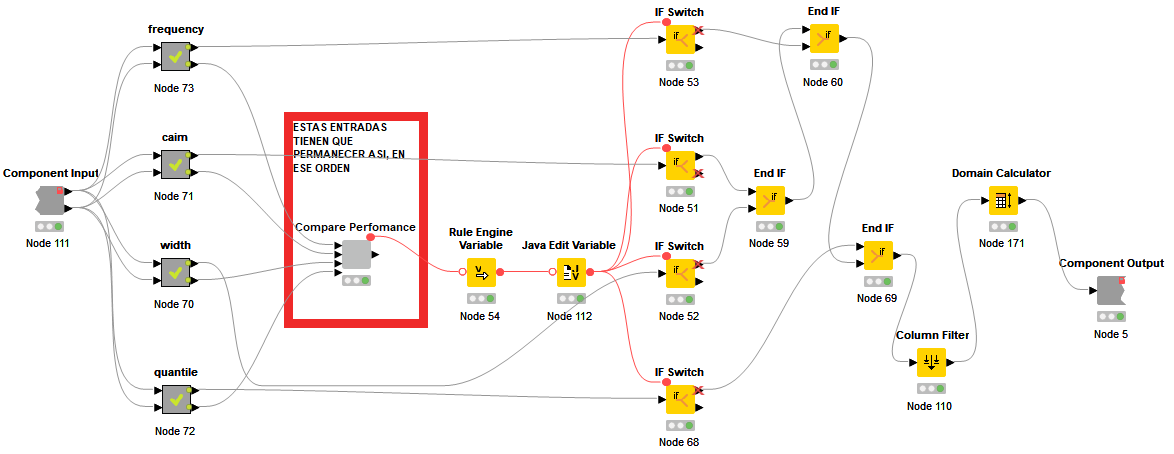
\includegraphics[width=\textwidth]{figuras/anexos/discretizer}
	\caption{Flujo KNIME del componente \textit{Discretizer}}
	\label{anex:discretizer}
\end{figure}


\chapter{Ejemplo de discretización \textit{Equal-Frequency} para el modelo ID3} \label{aped:9}
%\addcontentsline{toc}{section}{Anexo IX: Ejemplo de discretización\textit{Equal-Frequency} para el modelo ID3}

\begin{figure}[H]
	\centering
	\includegraphics[width=\textwidth]{"figuras/anexos/ejemplo discretizacion freq id3"}
	\caption{Flujo KNIME para la discretización\textit{ Equal-Frequency} en el modelo ID3}
	\label{anex:ejemplo-discretizacion-freq-id3}
\end{figure}

\chapter{Flujo KNIME del componente\textit{ MV Imputation}} \label{aped:10}
%\addcontentsline{toc}{section}{Anexo X: Flujo KNIME del componente \textit{MV Imputation}} 

\begin{figure}[H]
	\centering
	\includegraphics[width=\textwidth]{"figuras/anexos/MV Imputation"}
	\caption{Flujo KNIME del componente \textit{MV Imputation}}
	\label{anex:mv-imputation}
\end{figure}

\chapter{Flujo KNIME del componente \textit{Normalizer}} \label{aped:11}
%\addcontentsline{toc}{section}{Anexo XI: Flujo KNIME del componente \textit{Normalizer}}
	
\begin{figure}[H]
	\centering
	\includegraphics[width=\textwidth]{figuras/anexos/normalizer}
	\caption{Flujo KNIME del componente \textit{Normalizer}}
	\label{anex:normalizer}
\end{figure}
	

\chapter{Ejemplo de normalización \textit{Decimal Scaling} para el modelo PNN}\label{aped:12}
%\addcontentsline{toc}{section}{Anexo XII: Ejemplo de normalización \textit{Decimal Scaling} para el modelo PNN} \label{aped:12}

\begin{figure}[H]
	\centering
	\includegraphics[width=\textwidth]{"figuras/anexos/ejemplo normalizacion pnn decimal scaling"}
	\caption{Flujo KNIME para la normalización \textit{Decimal Scaling} en el modelo PNN}
	\label{anex:ejemplo-normalizacion-pnn-decimal-scaling}
\end{figure}

\chapter{Componente \textit{AutoML Clasificación}} \label{aped:13}
%\addcontentsline{toc}{section}{Anexo XII: Componente \textit{AutoML Clasificación}} 

\begin{figure}[H]
	\centering
	\includegraphics[width=\textwidth]{"figuras/anexos/componente integrado"}
	\caption{Flujo KNIME del componente \textit{AutoML Clasificación}}
	\label{anex:componente-integrado}
\end{figure}

\chapter{Ejemplo de integración de componentes al modelo PNN} \label{aped:14}
%\addcontentsline{toc}{section}{Anexo XIV: Ejemplo de integración de componentes al modelo PNN} 

\begin{figure}[H]
	\centering
	\includegraphics[width=\textwidth]{"figuras/anexos/ejemplo integracion componentes pnn"}
	\caption{Flujo KNIME de la integración de los componentes al modelo PNN}
	\label{fig:ejemplo-integracion-componentes-pnn}
\end{figure}


\chapter{Métodos de normalización elegidos acorde al \textit{dataset} y modelo} \label{aped:15-normalizacion}
En la tabla \ref{tabla-normalizacion} se muestra como tras la ejecución y evaluación de los normalizadores y de ejecutar el algoritmo de Aprendizaje Automático en cuestión, se escoge de forma automatizada el que mejor desempeño obtiene. Estos resultados destacan la influencia significativa del método de normalización en el rendimiento de los modelos de ML y cómo esta elección puede depender tanto del conjunto de datos específico como del algoritmo utilizado. 

\begin{table}
	\centering
	\caption{Métodos de normalización utilizados en cada \textit{dataset} para cada modelo}
	\label{tabla-normalizacion}
	\begin{tabular}{|l|l|l|} 
		\hline
		\textbf{\textit{Dataset}}                 & \textbf{Modelo} & \textbf{Método auto-seleccionado}  \\ 
		\hline
		\multirow{2}{*}{\textsc{dry bean}}        & PNN             & Z-score                            \\ 
		\cline{2-3}
		& SVM             & Z-score                            \\ 
		\hline
		\multirow{2}{*}{\textsc{human resources}} & PNN             & Decimal Scaling                    \\ 
		\cline{2-3}
		& SVM             & Z-score                            \\ 
		\hline
		\multirow{2}{*}{\begin{tabular}[c]{@{}l@{}}\textsc{water quality}\\\textsc{and potability}\end{tabular}} & PNN             & Z-score                            \\ 
		\cline{2-3}
		& SVM             & Decimal Scaling                    \\
		\hline
	\end{tabular}
\end{table}

\chapter{Métodos de discretización elegidos acorde al \textit{dataset} y modelo} \label{aped:16-discretizacion}
En la tabla \ref{tabla-discretizacion} se muestra como tras la ejecución y evaluación de los discretizadores y de ejecutar el algoritmo de Aprendizaje Automático en cuestión, se escoge de forma automatizada el que mejor desempeño obtiene. Estos resultados subrayan la variabilidad en la elección del método de discretización en función tanto del conjunto de datos como del modelo de aprendizaje automático. 

\begin{table}
	\centering
	\caption{ Métodos de discretización utilizados en cada \textit{dataset} para cada modelo}
	\label{tabla-discretizacion}
	\begin{tabular}{|l|l|l|} 
		\hline
		\textit{\textbf{Dataset}}                                                                                   & \textbf{Modelo} & \textbf{Método auto-seleccionado}  \\ 
		\hline
		\multirow{2}{*}{\textsc{cancer data}}                                                              & ID3    & CAIM                      \\ 
		\cline{2-3}
		& C4.5   & CAIM                      \\ 
		\hline
		\multirow{2}{*}{\begin{tabular}[c]{@{}l@{}}\textsc{academic} \\ \textsc{success} \end{tabular}}               & ID3    & Equal Frequency           \\ 
		\cline{2-3}
		& C4.5   &  Equal Frequency           \\ 
		\hline
		\multirow{2}{*}{\textsc{census income}}                                                            & ID3    & CAIM                      \\ 
		\cline{2-3}
		& C4.5   & Equal Width               \\ 
		\hline
		\multirow{2}{*}{\begin{tabular}[c]{@{}l@{}}\textsc{airline passenger} \\ \textsc{satisfaction} \end{tabular}} & ID3    & Equal Width               \\ 
		\cline{2-3}
		& C4.5   &  Equal Frequency           \\
		\hline
	\end{tabular}
\end{table}

\chapter{Métodos de imputación de valores faltantes elegidos acorde al \textit{dataset} y modelo} \label{aped:17-mv-imp}
En la tabla \ref{tabla-mv-imp-comparativa} se muestra como tras la ejecución y evaluación de los métodos de imputación de valores perdidos y de ejecutar el algoritmo de Aprendizaje Automático en cuestión, se escoge de forma automatizada el que mejor desempeño obtiene.
Estos resultados revelan la variabilidad en la elección de métodos de imputación de datos faltantes en función tanto del conjunto de datos específico como del modelo de aprendizaje automático. 


\begin{table}
	\centering
	\caption{Métodos de imputación de valores faltantes utilizados en cada \textit{dataset} para cada modelo}
	\label{tabla-mv-imp-comparativa}
	\begin{tabular}{|l|l|l|} 
		\hline
		\textbf{\textit{Dataset}}                                                                          & \textbf{Modelo} & \textbf{Método auto-seleccionado}  \\ 
		\hline
		\multirow{4}{*}{\textsc{human resources}}                                                          & ID3             & kMI                                \\ 
		\cline{2-3}
		& C4.5            & kMI                                \\ 
		\cline{2-3}
		& CART            & kMI                                \\ 
		\cline{2-3}
		& PNN             & kMI                                \\ 
		\hline
		\multirow{3}{*}{\textsc{census income}}                                                            & ID3             & kNNI                               \\ 
		\cline{2-3}
		& C4.5            & kNNI                               \\ 
		\cline{2-3}
		& CART            & kNNI                               \\ 
		\hline
		\multirow{6}{*}{\begin{tabular}[c]{@{}l@{}}\textsc{airline passenger} \\ \textsc{satisfaction} \end{tabular}} & ID3             & kMI                                \\ 
		\cline{2-3}
		& C4.5            & kMI                                \\ 
		\cline{2-3}
		& CART            & kNNI                               \\ 
		\cline{2-3}
		& PNN             & kNNI                               \\ 
		\cline{2-3}
		& RPROP           & kMI                                \\ 
		\cline{2-3}
		& SVM             & kNNI                               \\ 
		\hline
		\multirow{6}{*}{\begin{tabular}[c]{@{}l@{}} \textsc{water quality}\\\textsc{ and potability} \end{tabular}}    & ID3             & kMI                                \\ 
		\cline{2-3}
		& C4.5            & kMI                                \\ 
		\cline{2-3}
		& CART            & kNNI                               \\ 
		\cline{2-3}
		& PNN             & kMI                                \\ 
		\cline{2-3}
		& RPROP           & kMI                            \\ 
		\cline{2-3}
		& SVM             & kNNI                               \\
		\hline
	\end{tabular}
\end{table}


\end{document}